% !TeX program = pdflatex
% !TeX encoding = UTF-8
\documentclass[final,5p,times,twocolumn]{elsarticle}

\usepackage{amsmath,amssymb,mathtools}
\usepackage{booktabs,array,multirow}
\newcolumntype{C}[1]{>{\centering\arraybackslash}m{#1}}
\usepackage{graphicx,balance,makecell}
\usepackage{enumitem}
\usepackage{placeins}
\usepackage{stfloats}
\usepackage{float}
\usepackage{flafter}
\usepackage[expansion=false]{microtype}
  \usepackage{xurl}
\urlstyle{same}
  \usepackage{xcolor}
\definecolor{JMSCiteBlue}{HTML}{0072B2}
\usepackage[colorlinks=true,citecolor=JMSCiteBlue,linkcolor=JMSCiteBlue,urlcolor=JMSCiteBlue]{hyperref}
\graphicspath{{./}}
\setlength{\emergencystretch}{3em}
\setcounter{topnumber}{2}
\setcounter{dbltopnumber}{3}
\setcounter{dblbotnumber}{1}
\renewcommand{\topfraction}{0.90}
\renewcommand{\dbltopfraction}{0.72}
\renewcommand{\textfraction}{0.10}
\renewcommand{\floatpagefraction}{0.90}
\renewcommand{\dblfloatpagefraction}{0.95}

\journal{Journal of Manufacturing Systems}
\biboptions{numbers,sort&compress}

\newcommand{\cmax}{C_{\max}}
\newcommand{\pdi}{\mathrm{PDI}}
\newcounter{algorithm}
\newcommand{\algorithmtitle}[1]{\refstepcounter{algorithm}\noindent\textbf{Algorithm~\thealgorithm: #1}\par\smallskip}

\clubpenalty=10000
\widowpenalty=10000
\brokenpenalty=10000
\setlength{\textfloatsep}{10pt plus 2pt minus 2pt}
\setlength{\intextsep}{10pt plus 2pt minus 2pt}
\setlength{\floatsep}{8pt plus 2pt minus 2pt}
\setlength{\dbltextfloatsep}{10pt plus 2pt minus 2pt}
\setlength{\dblfloatsep}{8pt plus 2pt minus 2pt}
\hypersetup{pdftitle={Two-stage scheduling and structured solution methods for dual-source mixed-flow rotating-chamber cluster tools under full-occupancy processing},pdfauthor={Lizhen Shao; Lincong Wei; Wei Wang}}
\begin{document}
\raggedbottom
\begin{frontmatter}

\title{Two-stage scheduling and structured solution methods for dual-source mixed-flow rotating-chamber cluster tools under full-occupancy processing}
\author[ustb]{Lizhen Shao\corref{cor1}}
\ead{lshao@ustb.edu.cn}
\author[ustb]{Lincong Wei}
\author[ustb]{Wei Wang}
\cortext[cor1]{Corresponding author.}
\address[ustb]{Department of Control Science and Engineering, University of Science and Technology Beijing, No. 30 Xueyuan Road, Haidian District, Beijing 100083, China}

\begin{abstract}
Full-occupancy processing in rotating chambers requires every position to be occupied during production and cleaning. Reusable auxiliary wafers fill vacant positions, coupling processing and cleaning with a finite auxiliary inventory. For dual-source mixed-flow rotating-chamber cluster tools, this study develops a two-stage mixed-integer linear programming model using two-wafer pairs, termed PW pairs, to link transport and processing cycles and homogeneous product inventories to represent wafer sources. The model jointly determines pairing, chamber assignment, cleaning, and auxiliary-wafer reuse. It first minimizes product completion time and then refines waiting and production rhythm. A scheduling algorithm combines structured initialization with reinforcement-learning-based cut selection, using variable-role features and structure-aware reranking to improve time-limited search. Experiments show that structured initialization improves mixed-recipe schedules, while the complete cut-selection combination further reduces product completion time for continuous-processing and mixed-recipe instances in component comparisons with shared initial solutions. All 30 paired stage comparisons reduce total route waiting while preserving product completion time. In a single-product instance combining continuous processing and cleaning, total waiting decreases from 642 to 54~s. Paired comparisons of processing modes and auxiliary inventories reveal the dependence of continuous processing on auxiliary-wafer availability. An optimal two-product schedule with a completion time of 324~s and a feasible 16-product schedule with a completion time of 920~s demonstrate joint coordination of wafer processing and equipment timing.
\end{abstract}
\begin{keyword}
semiconductor manufacturing systems \sep cluster tools \sep dual-source material flow \sep mixed-integer linear programming \sep learning cut selection
\end{keyword}
\end{frontmatter}

\section{Introduction}
Plasma-enhanced chemical vapor deposition (PECVD) is an important process in semiconductor thin-film fabrication. Three-dimensional device structures and multilayer integration in advanced fabrication place greater demands on deposition uniformity and processing capability~\citep{appliedprecisioncvd}. Equipment manufacturers have developed multi-space process modules and multi-finger robots to support parallel processing within individual tools~\citep{gu2024applied,gu2024multifinger}. Cluster tools (CTs) connect process modules, robots, and load locks into continuous wafer-processing routes. Their feasible operating schedules depend jointly on processing and transport durations, load-lock switching, chamber cleaning, and residency constraints~\citep{pan2018survey}.

This study considers full-occupancy processing in rotating chambers for advanced fabrication, where reusable auxiliary wafers protect position bases during film processes with residues that are difficult to remove. Full occupancy during both production and cleaning is a process requirement. Auxiliary wafers occupy positions left vacant by products during production and fill all positions during cleaning, receiving deposited material and protecting the bases. They do not count toward product output and can be reused after return, but their handling, rotation, transport, and repeated loans consume equipment resources. Products enter through atmospheric load ports and reach the chambers via alignment and load locks. Auxiliary wafers enter from the atmospheric side in a single-source arrangement or from vacuum storage in a dual-source arrangement, forming mixed flows with products.

Four-position rotating chambers support $4\times1$ parallel processing and $2\times2$ chained processing. In the former, four wafers complete one processing exposure simultaneously. In the latter, paired loading, unloading, and rotation allow each product to undergo two consecutive exposures; auxiliary wafers at the beginning and end of a chain undergo one exposure. Both modes have the same total processing duration per product, but the two exposures and intervening rotation in chained processing create different loading and resource dependencies.



\begin{figure}[t]
\centering
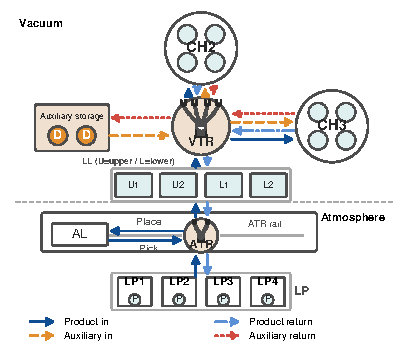
\includegraphics[width=\linewidth]{Figure1}
\caption{Topology and wafer routes of the dual-source mixed-flow rotating-chamber cluster tool.}
\label{fig:system-zh-new}
\end{figure}



Previous CT studies established analytical relationships among processing, transport, and throughput~\citep{perkinson1994throughput} and developed linear programming, heuristics, and timed Petri nets for residency-constrained scheduling~\citep{rostami2002optimal,wu2010closedform,qiao2012sojourn}. Subsequent work addressed wafer revisiting, multiple wafer types, and alternative process modules~\citep{qiao2014revisiting,wang2020multiple,wang2025virtualcell}. Clean- and dirty-hand allocation and steady-state cycle analysis for four-finger robots and four-space modules, together with joint optimization of the release and transport of two wafer types, provide a modeling basis for more complex tool structures~\citep{gu2024multifinger,yang2025miptwowafers}.

Periodic-cleaning scheduling coordinates production and cleaning through task-sequence enumeration, partial loading and timing control, dummy-wafer occupancy, and chamber-state triggers~\citep{kim2013cleaning,yu2020delay,qiao2022binary,li2022conditioncleaning}. Shared-buffer synchronization and dynamic action filtering address deadlock during module failures and noncyclic operation~\citep{zhu2025failuredeadlock,kim2025noncyclicdeadlock}. Waiting constraints also affect equipment output and upstream control~\citep{lee2018waiting}. Under full occupancy, cleaning changes production-chain boundaries, auxiliary-wafer occupancy, and vacuum-robot service sequences simultaneously. Scheduling product processing or cleaning times separately therefore does not capture all these dependencies.

Temporal quality in manufacturing systems also requires distinguishing batch efficiency from coordination between successive operations. Lee et al. relate allowable waiting to effective output~\citep{lee2018waiting}, whereas Weng et al. study just-in-time (JIT) scheduling to match job completion with downstream availability~\citep{weng2022jit}. In PECVD tools, reducing unnecessary waiting and coordinating the start intervals of repeated production cycles support predictable wafer supply and removal.

Equipment-data analysis, recipe-cycle anomaly detection, and predictive maintenance use operating data and process states to inform equipment-parameter updates~\citep{sun2024manufacturing,chen2020anomaly,biebl2020maintenance}. Variations in operation durations and differences among chambers and robots can change resource availability and require schedules to be recomputed after parameter updates~\citep{rahmani2014robust}. Here, operation durations are given inputs, and the focus is the scheduling interaction among recipes, cleaning, and dual-source wafer supply.

These wafer and resource constraints form a mixed-integer scheduling problem. Reinforcement learning can select CT actions or assist mixed-integer linear programming (MILP) search~\citep{kim2025adaptivecluster,tang2020cut,huang2022cutranking,paulus2022looking}. Wang et al. developed HEM, a hierarchical sequence model that coordinates the number of cuts and an ordered subset through reinforcement learning~\citep{wang2023hem}. We extend this framework with variable-role features and use structured initial solutions to improve the starting point of integer search.

Although existing studies cover multi-finger robots, multi-space modules, and cleaning, the joint arrangement of dual-source supply, full occupancy, reusable auxiliaries, and mixed recipes in rotating chambers further couples inventory, processing chains, and transport resources. For a PECVD CT with four-position rotating chambers, this study makes two contributions to batch organization and wafer-level scheduling:
\begin{enumerate}[leftmargin=*]
\item A two-stage MILP model uses PW pairs as transport and cycle-linking units and encodes products by batch jobs and source inventories. It jointly represents dual-source supply, full occupancy, continuous processing, cleaning, and finite auxiliary-wafer reuse. Product completion time is optimized first, followed by waiting and rhythm refinement with the principal structure retained; deterministic decoding then recovers individual-wafer schedules.
\item The RL-DMCT scheduling algorithm organizes primal-solution improvement and relaxation search. It constructs and progressively improves initial solutions using pairing, cycle, and resource structures, and extracts variable-role features to rerank candidate cuts using reinforcement-learning preferences, coverage, and representativeness.
\end{enumerate}
Section~2 formulates the rotating-chamber CT model. Section~3 presents RL-DMCT and wafer-schedule decoding. Section~4 reports the experiments, and Section~5 concludes the study.

\section{Scheduling model for rotating-chamber cluster tools}
\setcounter{equation}{0}
A processing cycle corresponds to one production exposure or one cleaning operation. A production cycle executes a product recipe. Cleaning uses only auxiliary wafers, and its threshold is at least two production cycles.

The model inputs are operation durations, resource capacities, residency limits, the cleaning threshold, and auxiliary inventory. Its outputs are resource assignments and operation start and end times for individual wafers. Tables~\ref{tab:symbol-cn-a} and~\ref{tab:symbol-cn-b} define the input constants and sets and the principal decision and auxiliary variables, respectively. Other notation is defined at first use. All times and durations are in seconds; quantities count wafers, pairs, or cycles.


\begin{table*}[!t]
\centering\small
\caption{Input parameters and sets for batch-job scheduling}
\label{tab:symbol-cn-a}
\renewcommand{\arraystretch}{1.03}
\setlength{\tabcolsep}{4pt}
\begin{tabular}{@{}C{0.20\textwidth}C{\dimexpr0.80\textwidth-8pt\relax}@{}}
\toprule
Symbol & Definition and value\\\midrule
$\mathcal J,\mathrm{Pjob}_j$ & $\mathcal J=\{1,\ldots,J\}$ is the batch-job set; $\mathrm{Pjob}_j$ is the set of products in job $j$.\\
$\mathcal L_j,\ell_{jk}$ & $\mathcal L_j$ lists the physical wafer identifiers of job $j$ in ascending order; $\ell_{jk}$ is the source LP of its $k$th product.\\
$N_{j\ell},N_j,N_\zeta,N_\psi,N$ & Product counts for job $j$ at LP $\ell$, job $j$ in total, the two production recipes, and the entire batch, respectively.\\
$m_j,\mathcal M,\mathcal C_j$ & $\mathcal M=\{\zeta,\psi,\mathrm{cl}\}$ denotes $4\times1$, $2\times2$, and cleaning, respectively; $m_j$ is the mode of job $j$. $\mathcal C=\{\mathrm{CH2},\mathrm{CH3}\}$ is the chamber set; nonempty $\mathcal C_j\subseteq\mathcal C$ gives the eligible chambers of job $j$.\\
$\mathcal P,\mathcal Q_c,\mathcal I$ & $\mathcal P=\{1,\ldots,P_{\max}\}$ is the PW-pair set; $\mathcal Q_c=\{1,\ldots,Q_{\max}\}$ is the cycle set for chamber $c$; $\mathcal I=\mathcal P\times\{0,1\}$ is the wafer-route task set.\\
$T,J_{\max},P_{\max},Q_{\max}$ & Upper bounds on tool-wide production cycles and cleaning operations, candidate PW pairs, and candidate cycles per chamber, respectively.\\
$\mathcal S,\sigma$ & $\mathcal S=\{A,V\}$ contains atmospheric and vacuum source regions. Source indicator $\sigma$ is 0 for single-source and 1 for dual-source supply.\\
$\mathcal O,\mathcal O^{\rm occ}$ & Candidate physical operations $\mathcal O$ and resource-occupancy intervals $\mathcal O^{\rm occ}$, generated from route and cycle templates.\\
$\mathcal R,K_\rho,\mathcal D$ & Resource set $\mathcal R$ and capacities $K_\rho$: ATR holds 2 wafers; VTR, 4; AL, 1; upper/lower LLs have 2 slots each; each chamber has 4 positions. Auxiliary set $\mathcal D=\{1,\ldots,D\}$ has default $D=8$; storage capacity is 10 wafers for two chambers.\\
$d_m\ (d_\zeta,d_\psi,d_{\mathrm{cl}})$ & Processing duration of type $m$; defaults $(d_\zeta,d_\psi,d_{\mathrm{cl}})=(180,90,500)$~s. Each $2\times2$ product requires two consecutive exposures.\\
$d_o^{\rm ATR},d_o^{\rm VTR},r_c$ & ATR handling, VTR handling, and chamber-$c$ half-turn durations; defaults are 4, 1, and 2~s, respectively.\\
$t_{\rm ATR},t_{\rm VTR},t_{\rm empty}$ & ATR exchange, VTR exchange, and empty ATR travel from LL to LP; defaults are 3, 2, and 6~s, respectively.\\
$t_{\rm AL},t_{\rm pump},t_{\rm vent}$ & Product alignment, upper-LL pumping, and lower-LL venting durations; defaults are 20, 30, and 25~s. Auxiliaries bypass AL.\\
$t_{\rm U}^{\rm reset},t_{\rm L}^{\rm reset}$ & Upper/lower LL-slot reset durations; defaults are 30 and 25~s, beginning after pickup from the opposite side is complete.\\
$d_o,\delta_{oo'},\delta^\rho_{oo'}$ & Duration of operation $o$, required interval from the end of $o$ to the start of $o'$, and repositioning/reset interval on resource $\rho$, respectively.\\
$H$ & Cleaning threshold $H\ge2$, with default $H=3$. Early cleaning is allowed after 1 to $H-1$ production cycles; cleaning is mandatory at $H$.\\
$\overline R_{i\rho}$ & Residency limit for route $i$ on resource $\rho$: placement end to pickup start in modules, with required exposure time deducted in chambers; pickup start to placement end on robots.\\
$B,M$ & Schedule horizon and conditional-constraint relaxation constant. Default $B=10000$~s includes LL reset completion; $M=B+\max\{\delta_{oo'},\delta^\rho_{oo'},r_c\}$.\\
$\lambda_1,\lambda_2,\lambda_3$ & Nonnegative weights for total waiting, maximum individual waiting, and rhythm variation; defaults $(\lambda_1,\lambda_2,\lambda_3)=(1,10,25)$.\\
$\varepsilon_C$ & Product-completion upper-bound tolerance; default $10^{-6}$~s.\\
\bottomrule
\end{tabular}
\end{table*}




\begin{table*}[t]
\centering\small
\caption{Principal decision and auxiliary variables}
\label{tab:symbol-cn-b}
\renewcommand{\arraystretch}{1.05}
\setlength{\tabcolsep}{4pt}
\begin{tabular}{@{}C{0.19\textwidth}C{0.18\textwidth}C{0.59\textwidth}@{}}
\toprule
Symbol & Type & Definition\\\midrule
$x_{j\ell pr}$ & Binary decision & Assigns a product of job $j$ at LP $\ell$ to position $r$ of pair $p$; defined when $N_{j\ell}>0$.\\
$v_p,\mu_{pm},z_{pc}$ & Binary decision & Pair activation, processing-type selection, and chamber assignment, respectively.\\
$X_{pcq},K_{cqm},f_{pcq}$ & Binary decision & Pair-$p$ occupancy of cycle $q$ in chamber $c$, cycle type, and pair placement on the accessible side, respectively.\\
$g_{pr\tau}$ & Binary decision & Assigns physical auxiliary $\tau\in\mathcal D$ to position $(p,r)$.\\
$h_{ou},y^\rho_{oo'},\gamma_{pa}$ & Binary decision & Selects unit $u$ for operation $o$, orders $o$ before $o'$ on resource $\rho$, and synchronizes both wafers of pair $p$ during handling segment $a$. Label $\mathrm{pick}$ denotes source-LP pickup.\\
$s_o,S_{cq}$ & Nonnegative real decision & Start times of operation $o$ and cycle $q$ in chamber $c$, respectively.\\
$e_o,b_o$ & Auxiliary & $e_o$ is the end time of $o$; binary $b_o$ indicates whether $o$ is active.\\
$\theta_{j\ell}$ & Nonnegative real auxiliary & Pickup-time boundary between consecutive nonempty LPs of job $j$.\\
$n_{cq}$ & Nonnegative integer auxiliary & Production cycles completed since the last cleaning after cycle $q$ of chamber $c$; range $0,\ldots,H$.\\
$F_p,F_p^\psi,X^P_{pcq}$ & Binary auxiliary & Product presence in pair $p$, presence of a $2\times2$ product, and product-containing pair occupancy of cycle $q$ in chamber $c$, respectively.\\
$\beta_{pr},d_{pr}$ & Binary auxiliary & Product assignment and auxiliary demand at position $(p,r)$, respectively.\\
$\chi_{iA},\chi_{iV}$ & Binary auxiliary & Atmospheric and vacuum supply indicators for route task $i$, respectively.\\
$C_{\max}$ & Nonnegative real decision & Upper bound on product return times to their original LPs.\\
$L_{\max},v_{cq}$ & Nonnegative real auxiliary & Upper bound on each waiting term and on absolute variation of adjacent cycle-start intervals centered at $(c,q)$, respectively.\\
\bottomrule
\end{tabular}
\end{table*}



\subsection{Batch-job and product-wafer encoding}
\label{sec:model-encoding-cn}
Products are grouped by processing mode, eligible chambers, and other scheduling attributes; each product belongs to exactly one batch job. Products of the same job at the same load port (LP) must have identical scheduling attributes to be represented by an inventory count. Different release times, processing requirements, or slot accessibility require separate jobs or explicit distinguishing constraints. The eligible chamber set can be $\{\mathrm{CH2}\}$, $\{\mathrm{CH3}\}$, or $\{\mathrm{CH2},\mathrm{CH3}\}$.

Slot $s$ of LP $\ell$ has physical wafer identifier $w=25(\ell-1)+s$. The identifiers of job $j$ are stored in ascending order in $\mathcal L_j$. Its $k$th product is denoted by $\mathrm{Pjob}_j[k]$, with source LP $\ell_{jk}$; these data determine inventory $N_{j\ell}$. Physical identities are recovered after optimization according to pickup order, as described in Section~\ref{sec:pjob-decoding-cn}.

A Pjob organizes product inventory by shared scheduling attributes. A PW pair contains two wafers and acts as a transport unit; a full-occupancy cycle processes two PW pairs simultaneously. The assignment and timing constraints in Section~\ref{sec:model-assignment-cn} enforce the within-job release order.

\subsection{Physical routes for single-source and dual-source mixed flows}
\label{sec:model-path-cn}
The source-region indicators are linked to wafer type and source arrangement $\sigma$ by
\begin{equation}
\begin{aligned}
\chi_{iA}&=\beta_{pr}+(1-\sigma)d_{pr},\\
\chi_{iV}&=\sigma d_{pr},\qquad i=(p,r)\in\mathcal I.
\end{aligned}
\label{eq:source-membership-cn}
\end{equation}
Equation~\eqref{eq:source-membership-cn} determines the source region of each wafer-route task. In the single-source arrangement, products are stored at LP1--LP4 and auxiliaries in atmospheric storage beside LP4. Both use the atmospheric transfer robot (ATR) and load-lock interfaces, while only products require alignment (AL). In the dual-source arrangement, products still originate from LP1--LP4, whereas auxiliaries are supplied from vacuum storage. Products follow the physical route in Fig.~\ref{fig:system-zh-new}.

Auxiliaries bypass AL. Single-source auxiliaries travel from atmospheric storage through ATR, the upper load lock (LL), and the vacuum transfer robot (VTR) to a process chamber, then return through VTR, the lower LL, and ATR. When supplied separately, they enter the LL directly without alignment. When accompanying a product, an auxiliary remains on ATR during product alignment, and the two enter the LL together after product pickup, as shown in Fig.~\ref{fig:single-source-cn}. Dual-source auxiliaries travel from vacuum storage to a chamber and back through VTR. These routes define the required physical operations; paired-transport choices and their timing conditions are given in Section~\ref{sec:model-time-cn}.


\begin{figure}[!htbp]
\centering
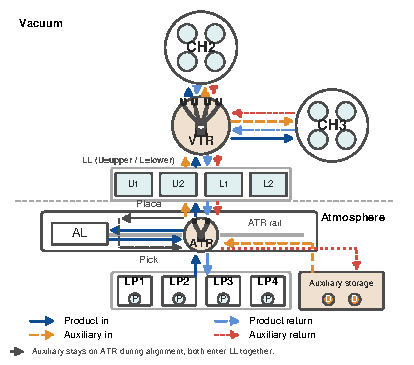
\includegraphics[width=\linewidth]{Figure2}
\caption{Topology and wafer routes of the single-source rotating-chamber cluster tool.}
\label{fig:single-source-cn}
\end{figure}



\subsection{Matching wafers, PW pairs, and chamber cycles}
\label{sec:model-assignment-cn}
The $4\times1$ mode replaces all four wafers between successive cycles. The $2\times2$ mode replaces two wafers and retains two for further processing. Wafers are therefore organized into PW pairs and assigned to compatible chambers and cycles. Each PW pair contains two wafers; position $r\in\{0,1\}$ is a pairing index, while physical carrying positions and chamber occupancy are determined by subsequent resource and cycle variables. Production and cleaning share candidate cycles. Exposure requirements and cleaning rules are specified in Section~\ref{sec:model-process-cn}.

\noindent\textbf{Wafer pairing and chamber selection.}
A PW pair can contain two products, one product and one auxiliary, or two auxiliaries. Every product must be processed, and each active pair position contains exactly one wafer:
\begin{equation}
\begin{aligned}
\sum_{p,r}x_{j\ell pr}&=N_{j\ell},\\
\beta_{pr}=\sum_{j,\ell}x_{j\ell pr},\qquad
\beta_{pr}+d_{pr}&=v_p.
\end{aligned}
\label{eq:joint-membership-cn}
\end{equation}
Equation~\eqref{eq:joint-membership-cn} enforces job inventories at each LP and exclusive occupancy of pair positions. Each position retains a complete processing route; physical product identities are recovered after optimization. An operation index $o$ can be written as $(i,a)$, $(p,a)$, or $(c,q,a)$, identifying an operation in a wafer route, PW pair, or chamber cycle, respectively. Here, $a$ is an operation label, and start and end times are denoted by $s_o,e_o$.

\noindent\textbf{Nondecreasing release order within each job.}
Under the specified release rule, products of a job at a lower-numbered LP must be picked up no later than products at its next nonempty LP. Let $h_j(\ell)=\min\{\ell'>\ell:N_{j\ell'}>0\}$ identify that next LP; no corresponding variable is created if the set is empty. For each position $(p,r)$, $o=((p,r),\mathrm{pick})$ denotes its LP pickup operation. Consecutive nonempty LPs satisfy
\begin{equation}
\begin{aligned}
0\le\theta_{j\ell}&\le B,\\
s_o&\le\theta_{j\ell}+M(1-x_{j\ell pr}),\\
s_o&\ge\theta_{j\ell}-M(1-x_{j,h_j(\ell),pr}).
\end{aligned}
\label{eq:pjob-release-boundary-cn}
\end{equation}
Equation~\eqref{eq:pjob-release-boundary-cn} orders pickups across LPs. Homogeneous products at the same LP are assigned physical identities by pickup time, ensuring nondecreasing release within each job. Products in the same PW pair and at the same LP may be picked up synchronously, subject to Eq.~\eqref{eq:stage-link-cn} and robot capacities. Other pickups obey ATR exclusion and repositioning constraints. Different Pjobs may interleave and may form pairs when their processing requirements are compatible.

Both wafers in a pair must have compatible processing modes and a jointly eligible chamber. Let $\mathcal C(m)\subseteq\mathcal C$ denote the chambers capable of processing type $m$. Mode and chamber selection satisfy
\begin{equation}
\begin{aligned}
\sum_m\mu_{pm}&=v_p,\qquad \sum_c z_{pc}=v_p,\\
x_{j\ell pr}&\le\mu_{p,m_j},\qquad
x_{j\ell pr}\le\sum_{c\in\mathcal C_j}z_{pc},\\
z_{pc}+\mu_{pm}&\le1\qquad(c\notin\mathcal C(m)).
\end{aligned}
\label{eq:joint-chamber-cn}
\end{equation}
Products from different jobs with the same mode may be paired, provided that the selected chamber belongs to the intersection of their eligible sets. A job eligible for both chambers may assign different PW pairs to different chambers.

Product presence, chained-processing status, and cleaning type satisfy
\begin{equation}
\begin{aligned}
F_p&\le\sum_r\beta_{pr}\le2F_p,\qquad F_p+\mu_{p,\mathrm{cl}}\le1,\\
F_p^\psi&\le F_p,\quad F_p^\psi\le\mu_{p\psi},\quad
F_p^\psi\ge F_p+\mu_{p\psi}-1.
\end{aligned}
\label{eq:pair-type-cn}
\end{equation}
The source and return LP of a product at $(p,r)$ are determined directly by $\sum_jx_{j\ell pr}$. Atmospheric and vacuum auxiliary sources are selected by $(1-\sigma)d_{pr}$ and $\sigma d_{pr}$, respectively.

\noindent\textbf{Candidate-capacity bounds.}
The following conservative bounds reserve sufficient candidates for joint pairing and cycle decisions:
\begin{equation}
\begin{gathered}
T=N_{\zeta}+2N_{\psi},\qquad J_{\max}=T,\\
P_{\max}=N+T+2J_{\max},\qquad Q_{\max}=T+J_{\max}.
\end{gathered}
\label{eq:candidate-bounds-cn}
\end{equation}
Every production cycle contains at least one product, so the number of production cycles is at most the total required exposures $T$. Each cleaning operation follows at least one production cycle, so at most $T$ cleaning operations are needed. Product-containing, production-filling, and cleaning pairs number at most $N$, $T$, and $2J_{\max}$, respectively. These bounds retain all admissible early-cleaning choices. PW-pair identifiers refer to occupancy tasks from loading to unloading and are counted separately from the inventory of reusable physical auxiliaries.

\noindent\textbf{Pair-to-cycle assignment.}
Both production and cleaning require four occupied chamber positions, so each active cycle contains exactly two PW pairs. Binary auxiliary variable $U_{cq}$ indicates whether cycle $q$ of chamber $c$ is active. Selected pairs must match the chamber and processing type of the cycle:
\begin{equation}
\begin{aligned}
\sum_mK_{cqm}&=U_{cq}, &\sum_pX_{pcq}&=2U_{cq},\\
X_{pcq}&\le z_{pc}, &X_{pcq}+\mu_{pm}&\le1+K_{cqm},\\
\sum_pX^P_{pcq}&\ge K_{cq\zeta}+K_{cq\psi}, &U_{c,q+1}&\le U_{cq},\\
\sum_{c,q}U_{cq}&\le Q_{\max}, &\sum_{c,q}K_{cq,\mathrm{cl}}&\le J_{\max}.
\end{aligned}
\label{eq:cycle-capacity-cn}
\end{equation}
Product-containing pair occupancy is linked by
\begin{equation}
X^P_{pcq}\le X_{pcq},\quad X^P_{pcq}\le F_p,\quad
X^P_{pcq}\ge X_{pcq}+F_p-1.
\label{eq:cycle-products-cn}
\end{equation}
Equation~\eqref{eq:cycle-capacity-cn} enforces full occupancy, pair--cycle compatibility, and candidate limits. Equation~\eqref{eq:cycle-products-cn} counts only product-containing pairs toward the production requirement. Each production cycle therefore contains at least one product pair, whereas cleaning contains only auxiliary pairs. Cycles are activated consecutively by index, while the sequence of processing modes remains a model decision.

\subsection{Operation timing and precedence}
\label{sec:model-time-cn}
Wafer operations obey route precedence, and paired transport additionally requires synchronized pickup and placement. Shared-resource service sequences are governed by Section~\ref{sec:model-resource-cn}.

\noindent\textbf{Operation activation and duration.}
Activation depends jointly on selected wafer routes, chamber cycles, and transport choices. Active operations have given durations; inactive operations have zero start and end times. LP pickup durations satisfy $d_o>0$. Thus,
\begin{equation}
0\le s_o\le B b_o,\qquad
0\le e_o\le B b_o,\qquad
e_o=s_o+d_ob_o.
\label{eq:operation-time-cn}
\end{equation}
Equation~\eqref{eq:operation-time-cn} fixes the durations of handling, alignment, pressure switching, rotation, and processing; waiting occurs only between operations. Product alignment is activated by $\beta_{pr}$, source-side, ATR, and LL operations by $\beta_{pr}+(1-\sigma)d_{pr}$, and VTR supply and return operations by $v_p$.

\noindent\textbf{Route-dependent precedence.}
Let $\mathcal A$ denote the active precedence arcs in common chamber-operation chains and wafer supply and return routes. Supply and return routes are activated according to source $\chi_{i\varsigma}$ and paired-transport or single-source accompanying choices, where $\varsigma\in\mathcal S$. For $(o,o')\in\mathcal A$, a successor starts after its predecessor ends and the required interval elapses; an active successor also requires an active predecessor:
\begin{equation}
b_{o'}\le b_o,\qquad
s_{o'}\ge e_o+\delta_{oo'}-M(2-b_o-b_{o'}).
\label{eq:precedence-cn}
\end{equation}
Equation~\eqref{eq:precedence-cn} connects loading, processing, and unloading on selected routes. Times lie in $[0,B]$, and $M$ covers the horizon and required intervals, relaxing conditional timing constraints when inactive.

\noindent\textbf{Stage linking and paired-operation synchronization.}
For operations $o,o'$ requiring synchronization, $x$ denotes the relevant existing binary variable for LP membership, cycle occupancy, or transport selection:
\begin{equation}
\begin{aligned}
-M(1-x)&\le s_o-s_{o'}\le M(1-x),\\
-M(1-x)&\le e_o-e_{o'}\le M(1-x).
\end{aligned}
\label{eq:stage-link-cn}
\end{equation}
Stage linking synchronizes individual-wafer operations with the corresponding operations of the selected physical batch. For paired transport, set $x=\gamma_{pa}$, $o=((p,0),a)$, and $o'=((p,1),a)$. The robot executes one common operation when synchronized, maintaining exclusion with other operations while the two wafers occupy separate carrying positions. Otherwise, the operations are ordered separately by Eq.~\eqref{eq:resource-order-cn}.

\noindent\textbf{Loading a single-source product--auxiliary pair.}
Route indices $i_{\rm P},i_{\rm D}$ identify the product and auxiliary routes, where $\mathrm P,\mathrm D$ are type labels. Binary variables $\gamma^{\rm early}_p,\gamma^{\rm late}_p,\gamma_{p,\mathrm{in}}$ select early auxiliary entry into the LL, auxiliary pickup after product placement on AL, or auxiliary entry together with the product. Operation labels $\mathrm{ALput,ALpick,LLput}$ denote placement on AL, retrieval from AL, and placement in the upper LL. Exactly one route is selected:
\begin{equation}
\begin{gathered}
\gamma^{\rm early}_p+\gamma^{\rm late}_p+\gamma_{p,\mathrm{in}}=1,\\
\gamma^{\rm early}_p=1\Rightarrow e_{(i_{\rm D},\mathrm{LLput})}\le s_{(i_{\rm P},\mathrm{ALput})},\\
\gamma^{\rm late}_p=1\Rightarrow s_{(i_{\rm D},\mathrm{pick})}\ge e_{(i_{\rm P},\mathrm{ALput})},\\
\gamma_{p,\mathrm{in}}=1\ \Longrightarrow
\begin{cases}
e_{(i_{\rm D},\mathrm{pick})}\le s_{(i_{\rm P},\mathrm{ALput})},\\
s_{(i_{\rm D},\mathrm{LLput})}=s_{(i_{\rm P},\mathrm{LLput})},\\
e_{(i_{\rm D},\mathrm{LLput})}=e_{(i_{\rm P},\mathrm{LLput})},\\
s_{(i_{\rm P},\mathrm{LLput})}\ge e_{(i_{\rm P},\mathrm{ALpick})}.
\end{cases}\end{gathered}
\label{eq:single-source-accompany-cn}
\end{equation}
For accompanying entry, ATR carries the auxiliary before placing the product on AL, then places both wafers into the upper LL after alignment. The auxiliary occupies an ATR carrying position continuously from source pickup to completion of LL placement. The product releases its ATR position while on AL and occupies a position again after retrieval. For separate auxiliary supply, source pickup is connected directly to LL entry.

\subsection{Processing modes and chamber cleaning}
\label{sec:model-process-cn}
Building on the pair--cycle assignments in Section~\ref{sec:model-assignment-cn}, this subsection specifies exposure counts, occupancy continuity, rotation and handling sequences, and cleaning boundaries. Time variables follow Section~\ref{sec:model-time-cn}.

\noindent\textbf{Production modes and continuous occupancy.}
Figures~\ref{fig:chain-zh} and~\ref{fig:parallel-zh} show the event sequences of the two modes. Cycle-occupancy constraints determine exposure counts and continuity.


\begin{figure}[t]
\centering
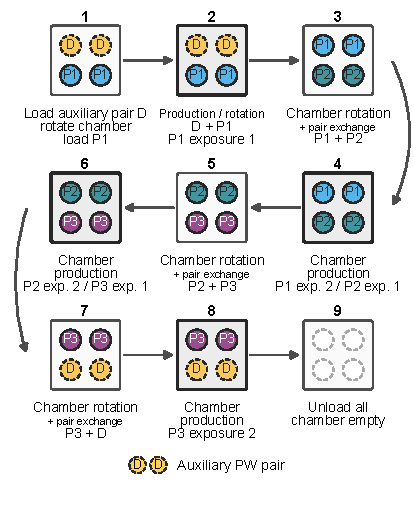
\includegraphics[width=0.89\linewidth]{Figure3}
\caption{Event sequence of $2\times2$ chained production. D denotes an auxiliary PW pair.}
\label{fig:chain-zh}
\end{figure}




\begin{figure}[t]
\centering
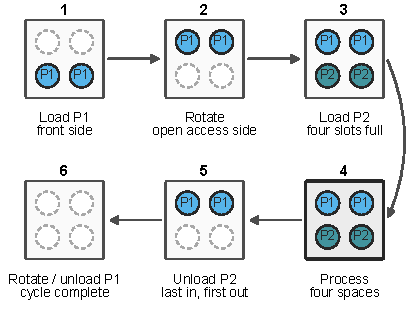
\includegraphics[width=\linewidth]{Figure4}
\caption{Event sequence of $4\times1$ parallel production.}
\label{fig:parallel-zh}
\end{figure}


Binary auxiliary variables $A_{pcq},Z_{pcq}$ indicate whether pair $p$ first and last participates in cycle $q$ of chamber $c$. Binary auxiliary variables $A^\psi_{pcq},Z^\psi_{pcq}$ identify these first and last participations for product-containing $2\times2$ pairs. With $X_{pc0}=X_{pc,Q_{\max}+1}=A_{pc,Q_{\max}+1}=0$ and direct substitution of $A_{pc1}=X_{pc1}$,
\begin{equation}
\begin{aligned}
A_{pcq}&\ge X_{pcq}-X_{pc,q-1}, &A_{pcq}&\le X_{pcq},\\
A_{pcq}&\le1-X_{pc,q-1},\\
Z_{pcq}&=X_{pcq}-X_{pc,q+1}+A_{pc,q+1},\\
\sum_{c,q}X_{pcq}&=v_p+F_p^{\psi}, &\sum_{c,q}A_{pcq}&=v_p,\\
A^{\psi}_{pcq}&=X_{pcq}-Z_{pcq}, &Z^{\psi}_{pcq}&=X_{pcq}-A_{pcq},\\
\sum_pA^{\psi}_{pcq}&\le1, &\sum_pZ^{\psi}_{pcq}&\le1.
\end{aligned}
\label{eq:cycle-exposures-cn}
\end{equation}
Equation~\eqref{eq:cycle-exposures-cn} makes every active pair enter a chamber once and participate in one or two consecutive cycles. The first three inequalities give $A_{pcq}=X_{pcq}(1-X_{pc,q-1})$, and the last-participation markers imply $\sum_{c,q}Z_{pcq}=\sum_{c,q}A_{pcq}=v_p$. A product-containing $4\times1$ pair receives one exposure; a product-containing $2\times2$ pair receives two consecutive exposures in the same chamber. Auxiliary-only filling and cleaning pairs participate in one cycle.

\noindent\textbf{Processing duration and cycle sequencing.}
A cycle starts only after its predecessor ends. Its duration depends on the selected type, giving end time $S_{cq}+\sum_m d_mK_{cqm}$:
\begin{equation}
\begin{aligned}
S_{cq}&\ge0,\\
S_{cq}+\sum_m d_mK_{cqm}&\le B U_{cq},\\
S_{cq}&\ge S_{c,q-1}+\sum_m d_mK_{c,q-1,m}\\
&\quad-M(1-U_{cq})\qquad(q>1).
\end{aligned}
\label{eq:cycle-time-cn}
\end{equation}
Processing durations are fixed, with waiting confined to intervals between operations. Handling and rotation durations are accounted for by separate events.

\noindent\textbf{Front/rear occupancy and rotating exchange.}
The robot accesses only the front side. A newly loaded pair occupies that side, while a pair retained from the previous cycle rotates to the rear. Binary auxiliary variables $\kappa_{cq},\upsilon_{cq}$ indicate whether cycle $q$ retains a pair from $q-1$ and whether both pairs leave after cycle $q$, respectively. Adjacent occupancies satisfy
\begin{equation}
\begin{aligned}
\kappa_{cq}&=\sum_p(X_{pcq}-A_{pcq}),\\
\upsilon_{cq}&=U_{cq}-\sum_p(X_{pcq}-Z_{pcq}),\\
f_{pcq}&\le A_{pcq},\qquad\sum_pf_{pcq}=U_{cq},\\
f_{pc,q-1}&\ge X_{pcq}-A_{pcq}\quad(q>1),\\
f_{pcq}&\ge F_p+K_{cq\psi}+X_{pcq}-2-\kappa_{cq}.
\end{aligned}
\label{eq:cycle-side-cn}
\end{equation}
Operations $(p,\mathrm{load})$ and $(p,\mathrm{unload})$ load and unload pair $p$. Operations $(c,q,\mathrm{rot-})$ and $(c,q,\mathrm{rot+})$ are half-turns before and after the cycle, activated by $U_{cq}$ and $\upsilon_{cq}$, each lasting $r_c$. Loading is linked by
\begin{equation}
\begin{aligned}
X_{pcq}=1\ \Rightarrow\quad
&S_{cq}\ge e_{(p,\mathrm{load})},\\
&s_{(p,\mathrm{unload})}\ge S_{cq}+\sum_m d_mK_{cqm};\\
A_{pcq}=1,\ f_{pcq}=0\ \Rightarrow\quad
&e_{(p,\mathrm{load})}\le s_{(c,q,\mathrm{rot-})};\\
A_{pcq}=1,\ f_{pcq}=1\ \Rightarrow\quad
&s_{(p,\mathrm{load})}\ge e_{(c,q,\mathrm{rot-})},\\
&S_{cq}=e_{(p,\mathrm{load})};\\
\kappa_{cq}=1\ \Rightarrow\quad
&s_{(c,q,\mathrm{rot-})}\ge S_{c,q-1}\\
&\qquad+\sum_m d_mK_{c,q-1,m}.
\end{aligned}
\label{eq:cycle-load-cn}
\end{equation}
If both pairs leave, the post-cycle rotation starts after processing ends. Unloading after the final exposure obeys
\begin{equation}
\begin{aligned}
Z_{pcq}=1,\ f_{pcq}=1\quad
&\Rightarrow e_{(p,\mathrm{unload})}\le s_{(c,q,\mathrm{rot+})},\\
Z_{pcq}=1,\ f_{pcq}=0,\ \upsilon_{cq}=1\quad
&\Rightarrow s_{(p,\mathrm{unload})}\ge e_{(c,q,\mathrm{rot+})},\\
Z_{pcq}=1,\ f_{pcq}=0,\ \upsilon_{cq}=0\quad
&\Rightarrow s_{(p,\mathrm{unload})}\ge e_{(c,q+1,\mathrm{rot-})}.
\end{aligned}
\label{eq:cycle-unload-cn}
\end{equation}
New pairs for the next cycle must wait until all departing pairs from the preceding cycle have been unloaded. For $p,p'\in\mathcal P$ and $q>1$,
\begin{equation}
\begin{aligned}
s_{(p',\mathrm{load})}&\ge e_{(p,\mathrm{unload})}\\
&\quad-M(2-Z_{pc,q-1}-A_{p'cq}).
\end{aligned}
\label{eq:cycle-exchange-cn}
\end{equation}
When one pair is retained, Eq.~\eqref{eq:cycle-exchange-cn} waits only for the replaced pair. When both depart, it waits for both unloads. Together with VTR exclusion, these constraints govern wafer exchange.

\noindent\textbf{Cleaning triggers and operation chains.}
A counter accumulates production cycles since the last cleaning and resets after cleaning. Cleaning is mandatory at the threshold and may occur earlier at admissible processing boundaries. Initial or consecutive cleaning operations are prohibited. With $U_{c,Q_{\max}+1}=0$,
\begin{equation}
\begin{aligned}
0\le n_{cq}&\le H U_{cq},\qquad n_{c0}=0,\\
K_{cq,\mathrm{cl}}=1&\Rightarrow n_{cq}=0,\\
U_{cq}=1,\ K_{cq,\mathrm{cl}}=0
&\Rightarrow n_{cq}=n_{c,q-1}+1,\quad n_{c,q-1}\le H-1,\\
K_{cq,\mathrm{cl}}=1&\Rightarrow 1\le n_{c,q-1}\le H,\\
n_{cq}&\le H-1+H U_{c,q+1}.
\end{aligned}
\label{eq:clean-counter-cn}
\end{equation}
Equation~\eqref{eq:clean-counter-cn} requires cleaning at the threshold, including after the final production segment. A zero initial count, a pre-cleaning count of at least one, and a reset after cleaning exclude initial and consecutive cleaning. Equations~\eqref{eq:cycle-capacity-cn} and~\eqref{eq:cycle-exposures-cn} require each chained product pair to participate in two consecutive production cycles, preventing intervening cleaning.

Cleaning is a full-occupancy cycle of type $m=\mathrm{cl}$ containing two auxiliary-only PW pairs. It uses the loading, unloading, and rotation rules of Eqs.~\eqref{eq:cycle-load-cn}--\eqref{eq:cycle-exchange-cn}: four auxiliaries are loaded on the two sides, cleaned, and unloaded in sequence. Intercycle links empty the chamber before and after cleaning. VTR exclusion and auxiliary loan--return constraints jointly determine transport and reuse times.

\subsection{Auxiliary reuse and robot and module resources}
\label{sec:model-resource-cn}
Physical resource availability is enforced through auxiliary identity assignment, robot carrying-position and module-slot allocation, occupancy exclusion, and residency limits.

\noindent\textbf{Auxiliary assignment and reuse.}
The two chambers share an auxiliary inventory. A wafer cannot be borrowed again until it has been returned. Each active loan request selects one physical wafer, and the two positions of a pair use different auxiliaries:
\begin{equation}
\sum_{\tau\in\mathcal D}g_{pr\tau}=d_{pr},\qquad
\sum_{r=0}^{1}g_{pr\tau}\le1.
\label{eq:dummy-assign-cn}
\end{equation}
Equation~\eqref{eq:dummy-assign-cn} assigns exactly one wafer to each auxiliary demand. Shared-resource constraints order loan intervals so that reuse follows return. They also apply across chambers, allowing parallel production with different auxiliary wafers.

\noindent\textbf{Robot and module capacities.}
Resource ordering distinguishes actuator exclusion from carrying-position capacity. ATR, VTR, AL, and each rotating chamber have exclusive actuator resources. Robot carrying positions, LL slots, and auxiliary identities are allocated as physical units with capacities from Table~\ref{tab:symbol-cn-a}. Chamber occupancy is already constrained by Eq.~\eqref{eq:cycle-capacity-cn}.

Each occupancy interval, whether a wafer-carrying assignment, auxiliary loan, or exclusive actuator use, selects an eligible unit. For an interval in $\mathcal O^{\rm occ}$, $\Gamma_o$ is its eligible-unit set, determined by wafer type and permitted operations. If eligibility depends on the selected wafer type, conditional constraints provide the corresponding link. Allocation satisfies
\begin{equation}
\sum_{u\in\Gamma_o}h_{ou}=b_o,\qquad 0\le s_o,e_o\le B.
\label{eq:slot-select-cn}
\end{equation}
Equation~\eqref{eq:slot-select-cn} assigns exactly one eligible unit to an active interval. The end time, including any reset tail, must remain within the common horizon. Paired wafers retain individual carrying-position occupancies, while Eq.~\eqref{eq:stage-link-cn} synchronizes operations. Equation~\eqref{eq:resource-order-cn} prevents overlapping occupancy of the same unit. If $\Gamma_o$ contains one unit, $h_{ou}=b_o$ can be substituted directly.

LL-slot occupancy starts with placement and ends after pickup and the subsequent reset. Reset restricts reuse of that slot and can overlap the robot's onward transport.

Physical hand identifiers $D_1,D_2,C_1,C_2$ denote VTR's two dirty and two clean hands. Unprocessed products use $\Gamma_o=\{D_1,D_2\}$; products that have completed all exposures use $\Gamma_o=\{C_1,C_2\}$. Both auxiliary supply and return permit $\Gamma_o=\{D_1,D_2,C_1,C_2\}$. A carrying task lasts from pickup start to placement completion, with the selected hand fixed throughout. Occupancies on the same hand are mutually exclusive under Eq.~\eqref{eq:resource-order-cn}, with zero repositioning interval for these carrying occupancies. Dirty and clean hands can each hold at most two wafers. Auxiliaries compete for free positions in both groups, and every carrying task must select a specific available hand.

\noindent\textbf{Resource exclusion and location-dependent repositioning.}
Resource precedence comprises given technical orders and service sequences to be decided. Route arcs follow processing requirements; resource-order variables coordinate other conflicting operations. When two occupancies select the same unit, one must start after the other ends and the repositioning or reset interval elapses:
\begin{equation}
\begin{aligned}
s_{o'}&\ge e_o+\delta^\rho_{oo'}-M(1-y^\rho_{oo'})
-M(1-h_{ou})-M(1-h_{o'u}),\\
s_o&\ge e_{o'}+\delta^\rho_{o'o}-My^\rho_{oo'}
-M(1-h_{ou})-M(1-h_{o'u}).
\end{aligned}
\label{eq:resource-order-cn}
\end{equation}
Equation~\eqref{eq:resource-order-cn} prevents overlapping use of the same unit; selecting different units permits parallel occupancy. It applies to robot operations, physical hands, module slots, chamber actuators, and individual auxiliaries.

Travel times are specified by location pairs. For operations whose chamber is selected through $z_{pc}$, the corresponding travel interval is activated for each candidate chamber combination. Let $p',c'$ denote another pair and its chamber, and let nonnegative constant $\delta^{\rm VTR}_{cc'}$ denote VTR travel time from $c$ to $c'$. For example, when both operations serve pairs $p,p'$ and are active,
\begin{equation}
\begin{aligned}
z_{pc}=z_{p'c'}=1,\ y^{\rm VTR}_{oo'}=1
\ \Rightarrow\ s_{o'}\ge e_o+\delta^{\rm VTR}_{cc'}.
\end{aligned}
\label{eq:location-travel-cn}
\end{equation}
Fixed-location operations use Eq.~\eqref{eq:resource-order-cn} directly. Product source and return locations are linked by $\sum_jx_{j\ell pr}$; travel intervals depend on the selected locations, and each product returns to its original LP.

\noindent\textbf{Residency limits and deadlock prevention.}
For an active route, $\operatorname{in}(i,\rho)$ and $\operatorname{out}(i,\rho)$ index placement into and pickup from module $\rho$. AL and LL limits apply directly between these endpoints. For a process chamber, required exposure time is subtracted before limiting nonprocessing residence. Required time includes production and cleaning, but excludes waiting, rotation, and handling; the exposure count is given by Eq.~\eqref{eq:cycle-exposures-cn}. For active route $i=(p,r)$,
\begin{equation}
\begin{aligned}
0\le\;&s_{\operatorname{out}(i,\rho)}-e_{\operatorname{in}(i,\rho)}
\le\overline R_{i\rho},\quad \rho\notin\mathcal C;\\
0\le\;&s_{(p,\mathrm{unload})}-e_{(p,\mathrm{load})}
-d_\zeta\mu_{p\zeta}\\
&-d_\psi(\mu_{p\psi}+F_p^\psi)
-d_{\mathrm{cl}}\mu_{p,\mathrm{cl}}\le\overline R_{i\rho},
\quad\rho\in\mathcal C.
\end{aligned}
\label{eq:residence-cn}
\end{equation}
The second group applies to the chamber actually visited. Occupancy ends, including reset tails, remain within $B$.

Precedence constraints~\eqref{eq:precedence-cn} and resource-order constraints~\eqref{eq:resource-order-cn} provide deadlock avoidance. For a candidate schedule, active operations form nodes, with directed arcs for operation precedence and solver-selected shared-resource orders. Circular waiting among robots, LLs, chambers, or auxiliaries would create a directed cycle. Summing the timing constraints around such a cycle of physical occupancy operations yields a positive duration or switching increment, requiring an operation to start strictly after itself. This contradicts temporal feasibility. Thus, for the given equipment parameters, schedules satisfying these constraints exclude circular waiting among the modeled operations and resources.

\subsection{Two-stage optimization with priority to product completion}
\label{sec:model-objective-cn}
Let $\mathcal F$ be the joint feasible region defined by the preceding constraints and $\xi$ the assignment of all retained model variables. Stage one minimizes product return completion time. Stage two preserves its upper bound and the principal discrete structure while optimizing waiting and production rhythm.

\noindent\textbf{Stage one: minimizing product return completion time.}
For position $(p,r)$, operation $o=((p,r),\mathrm{return})$ returns the wafer to its original LP. Only products impose lower bounds on the primary objective:
\begin{equation}
\begin{gathered}
C_{\max}\ge e_o-M(1-\beta_{pr})\quad(p,r),\\
\min_{\xi\in\mathcal F}C_{\max}.
\end{gathered}
\label{eq:primary-objective-cn}
\end{equation}
The makespan is the time when the last product completes its end-to-end route and returns to its LP. Cleaning between production segments affects $C_{\max}$ through subsequent product returns. Terminal cleaning remains in the equipment sequence but does not directly bound $C_{\max}$ when no product processing follows it. It may still compete for shared VTR capacity with products returning from another chamber, so its indirect effect depends on the complete schedule. The equivalent finite-batch output rate is $\mathrm{WPH}=3600N/C_{\max}$, measured in wafers per hour from batch start until the last product returns.

\noindent\textbf{Stage two: restricted timing refinement.}
Let $\widehat\xi$ be the best feasible stage-one assignment and $\widehat C$ its product completion time. Index set $\mathcal D_{\rm fix}$ includes components for pairing, chamber assignment, cycle occupancy, auxiliary identities, hand assignments, accompanying entry, and resource orders, excluding atomic synchronization choices that remain adjustable. Stage two adds
\begin{equation}
\begin{gathered}
\xi_d=\widehat\xi_d\quad(d\in\mathcal D_{\rm fix}),\qquad
C_{\max}\le\widehat C+\varepsilon_C.
\end{gathered}
\label{eq:secondary-domain-cn}
\end{equation}
Equation~\eqref{eq:secondary-domain-cn} fixes components $\xi_d=\widehat\xi_d$, while same-location atomic pickup/placement synchronization and continuous times remain adjustable.

Let $\mathcal W$ index waiting terms on supply and return routes. For term $\alpha$, $\omega_\alpha$ is the successor's start time minus the predecessor's end time and any required operation or travel duration. For every wafer, waiting includes the interval from VTR source-pickup completion to pair-loading start and from pair-unloading completion to VTR destination-placement start, after subtracting travel. Atmospheric routes additionally include interoperation intervals after deducting movement, alignment, pumping, or venting. For auxiliaries bypassing AL, the source-pickup-to-upper-LL-placement interval replaces the first three terms. All intervals run from a preceding end to a subsequent start. Chamber residence after processing and before unloading is governed by cycle, residency, and resource constraints; route waiting and in-chamber residence are recorded separately.

Total route waiting is $\sum_{\alpha\in\mathcal W}\omega_\alpha$, denoted by $L_{\rm sum}$ in the experiments. Both products and auxiliaries are included, and simultaneous waits of different wafers are counted separately. Maximum individual waiting satisfies
\begin{equation}
L_{\max}\ge\omega_\alpha\ge0,\qquad \alpha\in\mathcal W.
\label{eq:secondary-wait-cn}
\end{equation}
Set $\mathcal I_{\rm rhythm}$ contains the centers $(c,q)$ of three consecutive production cycles in the same $2\times2$ chain and chamber. A pair is retained at both adjacent boundaries, so $\kappa_{cq}=\kappa_{c,q+1}=1$; evaluation does not cross cleaning or chain boundaries. The set is determined once the cycle structure is fixed. The difference between successive start intervals is $S_{c,q+1}-2S_{cq}+S_{c,q-1}$, whose absolute value is bounded by
\begin{equation}
\begin{aligned}
v_{cq}&\ge S_{c,q+1}-2S_{cq}+S_{c,q-1},\\
v_{cq}&\ge-S_{c,q+1}+2S_{cq}-S_{c,q-1}
\quad((c,q)\in\mathcal I_{\rm rhythm}).
\end{aligned}
\label{eq:secondary-rhythm-cn}
\end{equation}
The weighted stage-two objective is
\begin{equation}
\begin{aligned}
\min\ \ &\lambda_1\sum_{\alpha\in\mathcal W}\omega_\alpha+\lambda_2L_{\max}\\
&+\lambda_3\sum_{(c,q)\in\mathcal I_{\rm rhythm}}v_{cq}.
\end{aligned}
\label{eq:secondary-objective-cn}
\end{equation}
Equation~\eqref{eq:secondary-objective-cn} combines total waiting, maximum individual waiting, and rhythm variation. With strictly positive corresponding weights and an optimal stage-two solution, $L_{\max}=\max_\alpha\omega_\alpha$ and $v_{cq}=|S_{c,q+1}-2S_{cq}+S_{c,q-1}|$. Experimental metrics are calculated from actual event times. Equally spaced starts of three consecutive production cycles have zero rhythm variation. Residency limits remain hard constraints.

\section{Reinforcement learning for dual-source mixed-flow cluster tool scheduling}
\label{sec:algorithm-cn}
We propose reinforcement learning for dual-source mixed-flow cluster tool scheduling (RL-DMCT) to search the combinatorial space defined by pairing, chamber cycles, and shared-resource orders. Its inputs are Pjobs, LP inventories, physical-identity mappings, and equipment parameters. It returns a wafer-level operation table and scheduling metrics, including product completion time.

RL-DMCT addresses time-limited solving through initial-solution improvement and cut-subset selection. Model-based initialization retains pairing, chamber assignments, and a cycle skeleton while progressively opening resource-order neighborhoods to improve the initial feasible upper bound. Structure-aware reranking uses the variable-role composition of cuts in both policy inputs and set evaluation, jointly considering policy preferences, role coverage, and candidate representativeness within the cut budget. Initialization improves primal solutions through schedule structure; cut selection uses constraint structure to organize the relaxation search. The two are combined in the main solve, followed by timing refinement and wafer-schedule decoding.

\subsection{Model-based structured initialization}
\label{sec:pjob-encoding-cn}
An initial solution is constructed from task assignments, PW pairs, and cycle links. Products are divided into consecutive segments and assigned to eligible chambers, paired according to mode, and supplemented with auxiliaries. Production cycles, continuous $2\times2$ chains, and cleaning boundaries are then arranged. Event times are assigned along supply, processing, and return routes using operation durations, robot travel, and resource-release times. The schedule is denoted by $\mathcal S^0$ after checking release order, resource occupancy, and residency conditions. Product pairs, auxiliary identities, chamber assignments, cycle occupancy, and event times are mapped to model variables; resource orders and logical auxiliary values complete the assignment $\xi^0=\mathsf{Enc}(\mathcal S^0)$. Here, $\mathsf{Enc}$ maps a physical schedule to a model assignment.

A structure-preserving binary skeleton (SPBS) improves $C_{\max}$ in progressively larger structural neighborhoods. The first layer fixes the principal discrete choices and adjusts continuous times and atomic pickup/placement synchronization. Subsequent layers release VTR orders, LL orders, and the remaining resource orders in turn. The final layer also releases cycle occupancy, front/rear positions, and hand assignments, while retaining pair composition, auxiliary identities, chamber assignments, inventory assignments, and cycle types. Let $t\in\{1,\ldots,5\}$ index layers and $\mathcal F_t$ the discrete components fixed in layer $t$. Relative to its starting assignment $\widehat\xi$, the temporary constraints are
\begin{equation}
\xi_d=\widehat\xi_d\quad(d\in\mathcal F_t),\qquad
\mathcal F_1\supseteq\cdots\supseteq\mathcal F_5.
\label{eq:spbs-fix-cn}
\end{equation}
Each layer uses at most one-fifth of the improvement budget and passes its best feasible assignment to the next layer. This first optimizes timing within a given structure, then adjusts resource orders to coordinate overlapping transport and processing, reducing the initial discrete search dimension. After full validation, the improved assignment initializes stage one and supplies a feasible upper bound; all temporary fixing constraints are removed. An existing feasible assignment can directly initialize SPBS. Construction and improvement costs are recorded separately from the main solve.

\subsection{Structure-aware reranking and reinforcement-learning-based cut selection}
\label{sec:hem-extension-cn}
Candidate cuts differ in separation strength and overlap in variable support and direction. RL-DMCT selects cuts through feature extraction, learned ordering, and structural reranking. Generic quality and variable-role information are extracted from the current MILP cuts; a reinforcement-learning policy selects the count and candidate order; structural coverage of the selected set guides subsequent additions. Learned ordering follows HEM's hierarchical count-control and ordered-subset framework~\citep{wang2023hem}. Variable-role representations are used in both policy inputs and reranking, allowing the cut budget to account for individual quality and complementarity.

\paragraph{Variable-role features}
Each cut has 13 generic features: objective parallelism, efficacy, support ratio, integer support, normalized violation, and the mean, maximum, minimum, and standard deviation of both cut and objective coefficients. Ten structural features are added using variable types and objective roles. Let $\mathcal V_a$ be the variables with nonzero coefficients in cut $a$, with coefficient $\alpha_{av}$ for variable $v$. Sets $\mathcal V_g$, $g\in\{1,\ldots,5\}$, denote binary, general integer, continuous objective, continuous auxiliary, and other variables, respectively. Continuous objective variables have nonzero objective coefficients. Role coefficient shares are
\begin{equation}
p_{ag}=\frac{\sum_{v\in\mathcal V_a\cap\mathcal V_g}|\alpha_{av}|}
{\sum_{v\in\mathcal V_a}|\alpha_{av}|}.
\label{eq:role-profile-cn}
\end{equation}
Absolute coefficients aggregate each role's contribution. Normalization removes positive row-scaling effects and is invariant to index permutations within a role. In this model, binary roles include pairing, chamber assignment, and resource ordering; continuous roles include objective quantities and event times. Roles are read directly from MILP variable attributes.

The remaining features are the coefficient shares of variables with finite lower and upper bounds, the positive-coefficient share, discrete--continuous coupling $\chi_a$, the largest identified-role share, and normalized role entropy $\mathcal H_a$, giving 23 inputs in total. In particular,
\begin{equation}
\begin{aligned}
\chi_a&=4(p_{a1}+p_{a2})(p_{a3}+p_{a4}),\\
\mathcal H_a&=-\frac{\sum_{g=1}^{5}p_{ag}\log p_{ag}}{\log5}.
\end{aligned}
\label{eq:role-information-cn}
\end{equation}
The coupling measure $\chi_a$ reflects joint participation of discrete choices and continuous timing: it equals one when the two groups each account for half the coefficient mass and zero when only one participates. Entropy $\mathcal H_a$ measures dispersion, ranging from zero for concentration in one role to one for a uniform distribution over five roles. Role shares describe composition, while coupling and entropy characterize cross-role interaction and concentration, distinguishing structurally different cuts with similar generic quality.

\paragraph{Learned ordering and candidate-pool construction}
The policy encodes the 23-dimensional features. Its upper level determines the number of cuts, and its lower level generates an ordered subset, with beam search retaining multiple candidate sequences. Let $k$ be the target count after applying solver limits. The policy sequence and a quality ranking are merged, deduplicated, and truncated to at most $2k$ candidates to form pool $\mathcal E$. Raw quality combines efficacy, violation, integer support, non-other-role share, largest identified-role share, and role entropy with weights 0.36, 0.24, 0.15, 0.15, 0.10, and $-0.05$, respectively. The first three terms are min--max normalized over candidates; the combined score is then normalized to $q_a\in[0,1]$, with zero assigned when the range is zero. Policy candidates enter first, followed by additional quality-ranked cuts.

\paragraph{Structural reranking by marginal gain}
Role shares define coverage, role concentration contributes to quality, and generic features together with role composition define candidate similarity. Let $\pi_a$ be a linearly decreasing prior score along the complete merged order, and let $d_g=\sum_{a\in\mathcal E}p_{ag}/\sum_{a\in\mathcal E,g}p_{ag}$ be role demand in the pool. Similarity $s_{ab}$ is the cosine similarity between vectors concatenating the first five generic features and the first four role shares, clipped to $[0,1]$, with diagonal entries equal to one. For selected set $A\subseteq\mathcal E$,
\begin{equation}
\begin{aligned}
G(A)={}&\sum_{a\in A}(0.35q_a+0.20\pi_a)\\
&+0.25\sum_gd_g\sqrt{\sum_{a\in A}p_{ag}}\\
&+\frac{0.20}{|\mathcal E|}\sum_{b\in\mathcal E}\max_{a\in A}s_{ba}.
\end{aligned}
\label{eq:cut-rerank-cn}
\end{equation}
The first term combines quality and policy preference. The second accumulates role coverage through a nondecreasing concave function, reducing the marginal benefit of further cuts once a role is well covered. The third is a facility-location representativeness term that covers different feature directions in the pool. Each term is monotone submodular, and their nonnegative weighted sum remains so~\citep{krause2014submodular}. A greedy marginal-gain rule therefore constructs the subset. With $G(\varnothing)=0$, the first $\lceil0.25k\rceil$ policy candidates are retained as anchors, capped by the actual policy output count. Candidates maximizing $G(A\cup\{a\})-G(A)$ are then added until the target count is reached.

Reranking evaluates both individual cut quality and its marginal contribution to the selected set. Diminishing returns balance role coverage, while representativeness reduces the incremental benefit of redundant candidates. Together with the policy prior, these terms determine selection order.

The policy is trained offline using HEM's hierarchical policy-gradient framework~\citep{wang2023hem}. The training set contains five existing scheduling MILPs with 4--12 products. Each epoch samples instances for eight solve attempts, with a 30~s main-solve limit per attempt. The upper level samples a cut ratio, and the lower level samples an ordered subset. The negative primal--dual integral of the main solve is the reward. Both policies use REINFORCE with an exponential-moving-average baseline coefficient of 0.9; the upper level is updated every two epochs. Training runs for 60 epochs, and the epoch-60 parameters are fixed when applied to the present model. Inference uses count prediction, beam search, and structural reranking without updating parameters.

Each inference considers at most 128 candidates and selects at most 16 cuts. The hidden dimension is 128 and the beam width is three; solver restrictions on forced cuts and selectable counts are preserved. The learned cut-selection component is denoted by RL-DMCT-S. Combined with SPBS, it forms the main RL-DMCT solution procedure. Ablations and comparison settings are defined in Section~\ref{sec:experiment-settings-cn}.

\subsection{Two-stage scheduling with RL-DMCT}
\paragraph{Stage one: joint adjustment of pairs, chambers, cycles, and resource orders}
Starting from validated initialization, the algorithm minimizes $C_{\max}$ over the complete feasible region $\mathcal F$ using Eq.~\eqref{eq:primary-objective-cn}. Search jointly adjusts pairing, eligible chamber assignments, cycle occupancy, cleaning positions, transport orders, and event times. Production segments are linked through shared VTR, LL, and auxiliary resources; transport and processing may overlap when processing and residency constraints permit. The incumbent is updated whenever a feasible schedule with earlier product completion is found. SCIP performs integer search~\citep{achterberg2009scip,bestuzheva2023scip}; RL-DMCT extracts structural features, invokes the trained policy, and reranks candidates at cut selection. At termination, a validated incumbent is recorded as $\widehat\xi$ with completion time $\widehat C$, together with a valid lower bound, gap, and stopping status. If refinement is enabled, the algorithm proceeds to stage two. Otherwise, or if no validated incumbent is found, it returns the corresponding schedule or no-incumbent status.

\paragraph{Stage two: timing refinement with the principal structure retained}
Starting from $\widehat\xi$, Eq.~\eqref{eq:secondary-domain-cn} fixes pairing, chamber assignment, cycle occupancy, auxiliary identities, hand assignments, and resource orders, and caps product completion at $\widehat C+\varepsilon_C$. Operation start times and atomic synchronization choices are adjusted to balance total waiting, maximum individual waiting, and same-chain start-interval variation through Eq.~\eqref{eq:secondary-objective-cn}. Supply and return operations and same-chain production starts are jointly adjusted under resource and residency constraints. A fully validated improvement replaces the stage-one schedule before decoding and output.

\subsection{Batch-job decoding and wafer-schedule output}
\label{sec:pjob-decoding-cn}
Let $\xi^\star$ be the final feasible assignment retained after construction, search, and refinement, and $\mathcal S^\star$ its wafer schedule. The decoding map $\mathsf{Dec}$ recovers physical identities and all event times through $\mathcal S^\star=\mathsf{Dec}(\xi^\star)$. For job $j$, positions satisfying $\sum_\ell x_{j\ell pr}=1$ are sorted by nondecreasing first LP pickup time, breaking ties by source LP, pair index, and within-pair position. Let $i_j^{(k)}$ be the $k$th sorted position. Identity recovery follows
\begin{equation}
i_j^{(k)}\longmapsto\mathrm{Pjob}_j[k]
\longmapsto\mathcal L_j[k],\qquad k=1,\ldots,N_j.
\label{eq:pjob-decoding-cn}
\end{equation}
Inventory and release-order constraints preserve source LPs, and tie-breaking makes the mapping deterministic. Recovered identifiers are attached to every event at their positions. Under the encoding conditions in Section~\ref{sec:model-encoding-cn}, decoding changes identities only: chamber assignments, resources, and event times are preserved, as are completion, waiting, and rhythm metrics.

The decoded operation table lists each wafer's source, pair, chamber, processing cycles, and all pickup and placement events. Resource occupancy is independently replayed on the same time axis. Validation checks that every product completes its required route and exposure count, auxiliary loan intervals do not conflict, robot, LL, and chamber capacities are respected, and release-order and residency conditions hold. Outputs include the wafer operation table, product completion, completion of all equipment operations, waiting and rhythm metrics, and stage-one bounds, gap, and stopping status.

\section{Computational experiments and results}
\label{sec:experiments-cn}
\subsection{Experimental settings and evaluation}
\label{sec:experiment-settings-cn}
The experiments address four questions: whether existing structure improves time-limited feasible upper bounds; how stage two reduces waiting and regulates rhythm; how continuous processing and auxiliary inventory affect completion time; and how much initialization and learned cut selection each contribute. An optimal two-product schedule and a feasible 16-product schedule then illustrate full occupancy, auxiliary filling, and shared-resource coordination. Paired comparisons use the same instance, initial schedule, and nominal solve budget. Default processing, transport, cleaning, and refinement parameters are given in Table~\ref{tab:symbol-cn-a}.

The platform runs Windows~11 with 20 logical processors and approximately 32~GB RAM, using Python~3.12.12 and PySCIPOpt~6.1.0. Each solve uses one thread. Every reported schedule passes full-model constraint checks and independent physical timing validation; metrics are calculated from wafer and equipment events. Solver-seed comparisons use seeds 1, 2, and 3, with means calculated within each instance. Multiple-training-seed comparisons additionally use training seeds 1, 2, and 3: each learned-method result aggregates nine runs, whereas SCIP aggregates three. Optimality is established from the bounds of the complete stage-one problem.

Comparisons include SCIP, HEM, RL-DMCT-S, and their SPBS combinations, plus three ablations: feature extension only, no structural reranking, and greedy decoding in place of beam search. Feature extension only uses an independently trained 23-input network and greedy sequence generation. The other two variants share the RL-DMCT-S parameters and change only the corresponding selection step. Root separation allows at most one separation round at the root and none elsewhere; normal separation retains SCIP's default settings.

Initialization and cut-selection comparisons in Sections~\ref{sec:algorithm-contribution-cn} and~\ref{sec:journal-transfer-cn} disable stage-two refinement and use a total nominal solve budget of 300~s. Without SPBS, all 300~s go to the main solve. With SPBS, 60~s improve initialization and 240~s remain for the main solve; unused initialization time is not transferred. SPBS uses the same nonlearning solver settings, and learned policies are used only in the subsequent main problem. Total elapsed time includes SPBS, the main solve, and validation; offline construction or search for the original input schedule is recorded separately.

Other stage budgets are specified in their respective subsections. Small-instance solves enable refinement after finding a feasible solution, whereas inventory and cleaning-rule comparisons solve only the primary problem. Time-limited comparisons report the best feasible result under the specified budget, with actual overruns stated separately.

\subsection{Using existing structure to reduce time-limited feasible upper bounds}
\label{sec:structure-comparison-cn}
This experiment evaluates whether existing schedule structure helps reduce product completion within a limited budget. Four dual-source mixed-recipe instances combine $N\in\{4,8\}$ and $H\in\{3,10\}$. Joint search, fixed initial structure, and fixed-then-joint search are compared in 36 runs. For each instance and seed, all strategies use the same initial schedule and a 300~s primary-solve budget; fixed-then-joint search allocates 60 and 240~s to its two parts. Offline initialization and model-construction times are recorded separately. Table~\ref{tab:structure-ablation-cn} compares product completion times.


\begin{table}[!htbp]
\centering\small
\caption{Search strategies for four mixed-recipe instances (three-seed means, s)}
\label{tab:structure-ablation-cn}
\begin{tabular}{ccccc}\toprule
$N$ & $H$ & Joint & Fixed & \makecell[c]{Fixed then\\joint}\\\midrule
4 & 3 & 854.53 & 543.67 & 647.00\\
4 & 10 & 854.53 & 542.00 & 542.00\\
8 & 3 & 2071.00 & 2029.33 & 2071.00\\
8 & 10 & 1720.00 & 1249.33 & 1575.00\\
\bottomrule\end{tabular}
\end{table}


As shown in Table~\ref{tab:structure-ablation-cn}, fixing structure produces lower mean feasible upper bounds than direct joint search in all four instances. For eight products and $H=10$, the mean decreases from 1720.00 to 1249.33~s. Fixed-then-joint search matches fixed-structure search only for four products and $H=10$ and has higher mean bounds in the other three cases. Within this 300~s budget, timing optimization around an existing structure is more effective than expanding discrete search. The joint model also provides valid lower bounds for the complete problem.

\subsection{Stage-two timing refinement and rhythm-weight ablation}
\label{sec:stage2-validation-cn}
Paired stage comparisons evaluate waiting before and after refinement of the same schedule, while preserving the product completion bound. A controlled weight ablation then fixes the stage-one input and varies only the rhythm weight to assess regulation of cycle-start intervals and its tradeoff with waiting.

\paragraph{Refinement of the same schedule with chamber eligibility restrictions}
Eight single- or dual-source mixed-recipe instances are each run with three seeds. Two additional eight-product instances assign different eligible chamber sets to Pjobs, giving 30 paired stage comparisons. Each run splits 300~s into 270~s for the primary problem and 30~s for refinement. Comparing stages within the same run controls for differences in primary-search trajectories. In the two restricted instances, some Pjobs can use only CH2, some only CH3, and others either chamber; each product must be processed in an eligible chamber.


\begin{table}[!htbp]
\centering\small
\caption{Timing refinement of the same schedule (three-seed means, s)}
\label{tab:refinement-ablation-cn}
\resizebox{\columnwidth}{!}{%
\begin{tabular}{ccccc}\toprule
$N/H$ & Supply / eligibility & $C_{\max}$ & Waiting before & Waiting after\\\midrule
4/3 & Single & 1491.00 & 1648.00 & 840.00\\
4/3 & Dual & 854.53 & 3991.73 & 333.67\\
4/10 & Single & 1491.00 & 1185.00 & 600.00\\
4/10 & Dual & 851.97 & 1259.65 & 626.67\\
8/3 & Single & 3933.00 & 3158.00 & 1680.00\\
8/3 & Dual & 2071.00 & 10943.00 & 536.00\\
8/10 & Single & 2985.00 & 2276.00 & 1200.00\\
8/10 & Dual & 1720.00 & 10998.02 & 692.00\\
8/3 & Single, restricted & 4707.00 & 3830.00 & 2040.00\\
8/3 & Dual, restricted & 2264.00 & 1046.00 & 341.00\\
\bottomrule\end{tabular}}
\end{table}


Table~\ref{tab:refinement-ablation-cn} compares mean total waiting before and after refinement. All 30 refined schedules pass physical replay and original-model assignment checks. Each retains product completion within tolerance and reduces total waiting. Individual reductions are 29.66\%--95.85\% in the 24 runs without additional chamber restrictions and 46.74\%--67.40\% in the six restricted runs. These reductions include auxiliary waiting unpenalized by the primary objective, showing that route waiting can be compressed without delaying product completion.

\paragraph{Controlled rhythm-weight ablation}
For a dual-source instance with 16 products, pure $2\times2$ processing, and $H=10$, each seed shares the same saved primary assignment across weights $\lambda\in\{0,5,25,100\}$. Each weight--seed combination receives 60~s of refinement. The objective sums total waiting, ten times maximum waiting, and $\lambda$ times rhythm deviation. The principal discrete structure and completion bound are identical.


\begin{table}[!htbp]
\centering\small
\caption{Rhythm-weight ablation (three-seed means, times in s)}
\label{tab:rhythm-weight-cn}
\begin{tabular}{ccccc}\toprule
Instance & $\lambda$ & $C_{\max}$ & \makecell[c]{Total\\waiting} & \makecell[c]{Rhythm\\deviation}\\\midrule
\multirow[c]{4}{*}{\makecell[c]{16 products\\$2\times2$}} & 0 & 2537 & 1000 & 792\\
 & 5 & 2537 & 1016 & 784\\
 & 25 & 2537 & 1016 & 784\\
 & 100 & 2537 & 1016 & 784\\
\bottomrule\end{tabular}
\end{table}


As Table~\ref{tab:rhythm-weight-cn} shows, adding the rhythm term decreases deviation from 792 to 784~s, increases total waiting from 1000 to 1016~s, and preserves product completion at 2537~s. Weights 5, 25, and 100 yield identical metrics, selecting the same waiting--rhythm tradeoff for this structure.

\subsection{Coupled effects of continuous processing, cleaning, and auxiliary inventory}
\label{sec:coupled-effects-cn}
Small-instance bounds first establish solution quality. The processing, cleaning, and loan--return events of a single-product $2\times2$ schedule are then examined. Paired inventory and cleaning-rule experiments explain completion-time differences. Optimal values, event sequences, and parameter comparisons jointly evaluate the model's representation of the coupled constraints.

\subsubsection{Small-instance optima and timing improvements between stages}
Table~\ref{tab:default-small-new-cn} reports four small instances. The primary budget is 600~s, followed by 60~s of refinement after a feasible solution is obtained. Primary optimality is proved in all four.


\begin{table}[!htbp]
\centering\small
\caption{Complete solution results for small instances (s)}
\label{tab:default-small-new-cn}
\resizebox{\columnwidth}{!}{%
\begin{tabular}{cccc}\toprule
$N$/Recipe/$H$ & LP distribution & Lower/upper bound & Waiting: before$\to$after\\\midrule
1/$4\times1$/3 & LP1 & 296.00/296.00 & $198\to6$\\
1/$2\times2$/2 & LP1 & 303.00/303.00 & $642\to54$\\
2/$4\times1$/3 & Across LPs & 324.00/324.00 & $72\to47$\\
2/$4\times1$/3 & Same LP & 324.00/324.00 & $244\to56$\\
\bottomrule\end{tabular}}
\end{table}


The one-product $2\times2$, $H=2$ instance in Table~\ref{tab:default-small-new-cn} combines continuous processing, cleaning, and auxiliary reuse. In Fig.~\ref{fig:d-coupled-witness-cn}, the same product-containing pair participates in adjacent CH2 cycles at $[76,166]$ and $[170,260]$~s, totaling 180~s of processing. It remains inside the chamber between exposures while rotation and exchange take place. The second cycle reaches $H=2$, triggering cleaning with four auxiliaries at $[284,784]$~s and resetting the counter. Lanes D1--D7 show nine complete loan intervals across seven physical identities. D2 and D3 both return at 173~s and are borrowed again for cleaning at 270 and 273~s, respectively, without overlapping loans. Peak simultaneous borrowing is five wafers; D8 is unused.


\begin{table}[!htbp]
\centering\small
\caption{Stage metrics for the continuous-processing and cleaning schedule (times in s)}
\label{tab:d-coupled-witness-cn}
\setlength{\tabcolsep}{3pt}
\begin{tabular}{ccc}\toprule
Metric & Stage one & After refinement\\\midrule
Product completion & 303 & 303\\
Total waiting & 642 & 54\\
Maximum individual waiting & 96 & 16\\
End of all occupancy & 978 & 796\\
Production/cleaning cycles & 2/1 & 2/1\\
Loans/physical auxiliaries & 9/7 & 9/7\\
Repeat loans/peak simultaneous loans & 2/5 & 2/5\\
Valid rhythm centers & 0 & 0\\\bottomrule
\end{tabular}
\end{table}




\begin{figure}[!htbp]
\centering
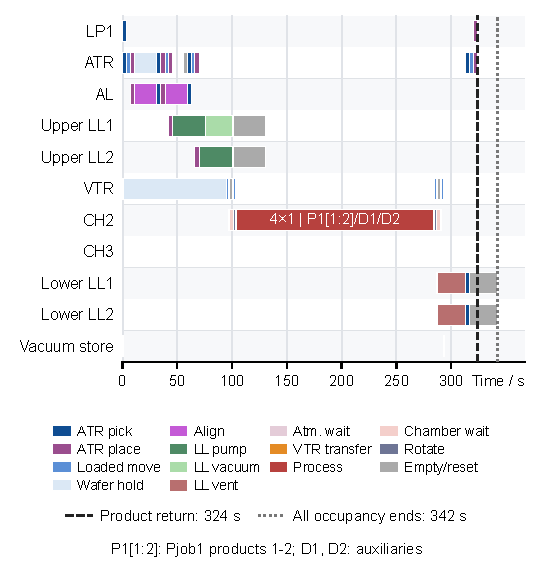
\includegraphics[width=\columnwidth]{Figure5}
\caption{Continuous product processing and auxiliary loan intervals. The top lane shows the two $2\times2$ product exposures. Blue and green intervals on D1--D7 denote loans for production and cleaning, respectively. Dashed and dotted lines mark product completion at 303~s and the end of all occupancy at 796~s.}
\label{fig:d-coupled-witness-cn}
\end{figure}


Table~\ref{tab:d-coupled-witness-cn} shows that fixed-structure refinement reduces total waiting from 642 to 54~s and the end of all occupancy from 978 to 796~s while preserving the proven optimal product completion. Cleaning and auxiliary returns continue after the product returns, so post-return equipment occupancy is also reported. Auxiliary return and reuse connect continuous processing with full-occupancy cleaning. The next comparison varies auxiliary inventory and cleaning rules to assess their effects on product completion.

\subsubsection{Effect of auxiliary inventory on continuous-processing completion}
\label{sec:journal-mechanism-cn}
The scenarios comprise one product under pure $4\times1$ or pure $2\times2$ processing, two products with mixed recipes, and four products under each of three recipe patterns. Crossing these with $H\in\{2,3\}$ and $|\mathcal D|\in\{4,8\}$ gives 24 instances. Each compares optional early cleaning against threshold-based cleaning. The latter permits cleaning only when the production count reaches $H$, or when it is $H-1$ and the next cycle uses $2\times2$ processing. Three solver seeds per rule yield 144 runs. Both rules use the same full candidate space and a common feasible initial schedule when available; otherwise, both start without an incumbent. The nominal main-solve budget is 600~s, with refinement disabled.


\begin{table}[!htbp]
\centering\small
\caption{Optimal product completion for single-product scenarios (s)}
\label{tab:journal-mechanism-cn}
\begin{tabular}{cccc}\toprule
$H$ & Auxiliaries & Pure $4\times1$ & Pure $2\times2$\\\midrule
2 & 4 & 296 & 309\\
2 & 8 & 296 & 303\\
3 & 4 & 296 & 309\\
3 & 8 & 296 & 303\\
\bottomrule\end{tabular}
\end{table}


Table~\ref{tab:journal-mechanism-cn} shows that increasing auxiliary inventory from four to eight reduces the optimal $2\times2$ completion by 6~s, or 1.94\%, under both thresholds and cleaning rules. The $4\times1$ optimum remains 296~s. Inventory effects therefore depend on the processing route: even with equal cumulative exposure time, loading, unloading, rotation, and auxiliary availability change the optimum. In these single-product cases, $4\times1$ completes 13 or 7~s earlier than $2\times2$.

The $2\times2$, $H=2$ cases yield 11 valid schedules containing continuous processing, full-occupancy cleaning, and auxiliary reuse. All five schedules with inventory four use four identities for nine loans, including five repeat loans. This supports joint representation of loan--return timing and cleaning occupancy under finite inventory. Increasing $H$ from two to three removes the single cleaning operation, while the optimal product completion remains 309 and 303~s for the two inventories. This distinguishes product completion from post-batch cleaning occupancy.

\subsection{Contributions of structured initialization and learned cut selection}
\label{sec:algorithm-contribution-cn}
Four dual-source instances with feasible initial schedules are used: two products under pure $4\times1$ processing across LPs or within one LP, two products with mixed recipes and $H=3$, and four products with mixed recipes and $H=10$. Initial completion times are 324, 324, 518, and 542~s, respectively. Comparisons within each instance share the original schedule and examine structural search, SPBS and cut selection, and training-seed effects in turn.

\subsubsection{Complementarity of fixed-structure optimization and subsequent joint search}
\label{sec:journal-structure-cn}
Joint search, fixed original structure, and fixed-then-joint search are compared in 36 runs. The nominal primary budget is 300~s, split into 60+240~s for fixed-then-joint search. Unused fixed-stage time is not added to joint search.


\begin{table}[!htbp]
\centering\small
\caption{Search strategies for four small dual-source instances (three-seed mean product completion, s)}
\label{tab:journal-structure-cn}
\setlength{\tabcolsep}{3pt}
\begin{tabular}{cccc}\toprule
Instance & Joint & Fixed & \makecell[c]{Fixed then\\joint}\\\midrule
2 products/$4\times1$/\makecell[c]{Across\\LPs} & 324 & 324 & 324\\
2 products/$4\times1$/Same LP & 324 & 324 & 324\\
2 products/Mixed/$H=3$ & 513.34 & 507.00 & 505.67\\
4 products/Mixed/$H=10$ & 542 & 542 & 542\\
\bottomrule\end{tabular}
\end{table}


Mean completion times are given in Table~\ref{tab:journal-structure-cn}. For the two-product mixed instance, all three fixed-structure runs reach the restricted optimum of 507~s, with mean total elapsed time 3.37~s. Fixed-then-joint search obtains a best feasible value of 503~s, a mean of 505.67~s, and mean elapsed time 243.65~s. Direct joint search gives a mean upper bound of 513.34~s and elapsed time 300.73~s. Thus, fixed-structure optimization quickly lowers the initial upper bound, and subsequent discrete adjustment improves it further. The other three instances have identical final objectives across strategies: both pure $4\times1$ cases reach the complete-problem optimum of 324~s, and the four-product mixed case retains its feasible bound of 542~s.

Together with Section~\ref{sec:structure-comparison-cn}, these results show that an existing structure provides an effective timing-optimization starting point, while the benefit of releasing discrete decisions depends on the instance. In the two-product mixed case, structural adjustment improves even an optimal schedule of the fixed-structure subproblem.

\subsubsection{Initialization gains and the influence of separation settings}
\label{sec:journal-ablation-cn}


\begin{table*}[!t]
\centering\small
\caption{SPBS and cut selection: training seed 1 and three solver seeds (mean product completion, s)}
\label{tab:journal-algorithm-cn}
\setlength{\tabcolsep}{3.5pt}
\begin{tabular}{cccccccc}\toprule
Instance & Separation & SCIP & HEM & RL-DMCT-S & SCIP+SPBS & HEM+SPBS & RL-DMCT\\\midrule
\multirow[c]{2}{*}{2 products/$4\times1$/Across LPs} & Root & 324 & 324 & 324 & 324 & 324 & 324\\
 & Normal & 324 & 324 & 324 & 324 & 324 & 324\\
\multirow[c]{2}{*}{2 products/$4\times1$/Same LP} & Root & 324 & 324 & 324 & 324 & 324 & 324\\
 & Normal & 324 & 324 & 324 & 324 & 324 & 324\\
\multirow[c]{2}{*}{2 products/Mixed/$H=3$} & Root & 513.34 & 514.02 & 512.00 & 505.00 & 503.67 & 505.00\\
 & Normal & 516.67 & 516.75 & 518.00 & 509.00 & 508.67 & 505.00\\
\multirow[c]{2}{*}{4 products/Mixed/$H=10$} & Root & 542.00 & 542.00 & 542.00 & 541.00 & 541.00 & 541.00\\
 & Normal & 542.00 & 542.00 & 542.00 & 541.00 & 541.00 & 541.00\\
\bottomrule\end{tabular}
\end{table*}


With training seed one, initialization and cut selection are compared under root and normal separation. Normal separation evaluates six methods in 72 runs. Root separation adds three ablations without SPBS, giving 108 runs. Section~\ref{sec:journal-training-cn} adds training seeds to assess consistency.

All 180 runs yield feasible schedules. The two pure $4\times1$ instances are solved to optimality, whereas the mixed instances yield time-limited feasible solutions. In the root-separation, four-product mixed SCIP comparison without SPBS, solver seed one takes 428~s of actual main-solve time.

Table~\ref{tab:journal-algorithm-cn} shows that the pure $4\times1$ objectives cannot improve further; differences concern the time to prove optimality. For the two-product mixed case under root separation, SPBS reduces every seed's starting value from 518 to 505~s, a 2.51\% reduction. Subsequent HEM search reaches 501~s in one seed, producing a mean upper bound of 503.67~s. Under normal separation, SPBS outputs 511, 505, and 511~s; subsequent RL-DMCT-S search gives 511, 501, and 503~s. Its mean of 505~s is below 508.67~s for HEM+SPBS, reversing the root-separation ranking. For the four-product mixed case, SPBS reduces 542 to 541~s under both settings, a 0.18\% reduction, with no further main-solve improvement. Thus, SPBS improves mixed-instance starting points, while additional cut-selection gains occur in particular instances and seeds and vary with separation settings.

In root-separation ablations without SPBS, all methods reach 324~s on both pure-recipe instances and average 542~s on the four-product mixed instance. For two mixed products, RL-DMCT-S averages 512.00~s, compared with 516.00~s without structural reranking, 511.00~s with greedy decoding instead of beam search, 515.33~s with feature extension only, and 514.02~s for HEM. Structural reranking reduces the mean by 4~s in this comparison, whereas greedy decoding improves on beam search by 1~s. Section~\ref{sec:journal-transfer-cn} compares components across training seeds under normal separation and shared initialization.

Normal separation produces 0--250 HEM callbacks and 2--224 RL-DMCT-S callbacks per run, compared with 0--2 learned calls under root separation for these methods and their SPBS combinations. Despite more callbacks, HEM and RL-DMCT-S without SPBS have higher mean bounds on the two-product mixed instance under normal separation. For the two pure $4\times1$ cases under normal separation without SPBS, mean main-solve times for SCIP, HEM, and RL-DMCT-S are 69.00, 50.67, and 51.67~s across LPs and 37.33, 12.67, and 52.67~s within one LP. Corresponding total elapsed means are 71.14, 54.36, and 55.05~s and 39.36, 16.16, and 55.52~s.

For the two-product mixed instance, mean total elapsed times of SCIP+SPBS, HEM+SPBS, and RL-DMCT range from 250.46 to 251.86~s under root separation and from 255.60 to 257.64~s under normal separation. Product completion and equipment occupancy can change differently. For four mixed products under normal separation, adding SPBS reduces product completion from 542 to 541~s but extends the end of all occupancy from 553 to 591~s, reflecting the occupancy tail under a product-return objective.

\subsubsection{Consistency of initialization gains across training seeds}
\label{sec:journal-training-cn}
Adding training seeds two and three to normal-separation comparisons gives 168 runs: 72 shared with the preceding experiment and 96 additional runs. HEM and RL-DMCT-S each account for 72 runs, and SCIP for 24. Results follow the aggregation defined in Section~\ref{sec:experiment-settings-cn}. Both pure $4\times1$ cases retain the proven optimum of 324~s. Table~\ref{tab:journal-training-cn} reports the mixed instances.


\begin{table}[!htbp]
\centering\small
\caption{Initialization across training seeds under normal separation (mean product completion, s)}
\label{tab:journal-training-cn}
\begin{tabular}{cccc}\toprule
Instance & Method & Without SPBS & With SPBS\\\midrule
\multirow[c]{3}{*}{2 productsMixed} & SCIP & 516.67 & 509.00\\
 & HEM & 517.14 & 508.89\\
 & RL-DMCT-S & 517.44 & 507.67\\
\multirow[c]{3}{*}{4 productsMixed} & SCIP & 542.00 & 541.00\\
 & HEM & 542.00 & 541.00\\
 & RL-DMCT-S & 542.00 & 541.00\\
\bottomrule\end{tabular}
\end{table}


Table~\ref{tab:journal-training-cn} shows that SPBS improves mean completion for every method on both mixed instances, with the same direction across all three training seeds. For two mixed products, each training seed uses SPBS inputs of 511, 505, and 511~s. RL-DMCT means by training seed are 505, 509, and 509~s, compared with 508.67, 509, and 509~s for HEM+SPBS. Additional cut-selection improvement over HEM+SPBS occurs in training seed one. For four mixed products, all training seeds improve from 542 to 541~s through initialization. One HEM+SPBS run and one RL-DMCT run have actual main-solve times of 245 and 243~s, respectively.

\subsection{Initialization and cut-selection gains under supply and inventory changes}
\label{sec:journal-transfer-cn}


\begin{table*}[!t]
\centering\small
\caption{Algorithms across recipes and supply scenarios (mean product completion, s)}
\label{tab:journal-transfer-cn}
\begin{tabular}{cccccccc}\toprule
Recipe & Scenario & SCIP & HEM & RL-DMCT-S & SCIP+SPBS & HEM+SPBS & RL-DMCT\\\midrule
$4\times1$ & S1 & 324.00 & 324.00 & 324.00 & 324.00 & 324.00 & 324.00\\
$4\times1$ & S2 & 324.00 & 324.00 & 324.00 & 324.00 & 324.00 & 324.00\\
$4\times1$ & S3 & 324.00 & 324.00 & 324.00 & 324.00 & 324.00 & 324.00\\
$2\times2$ & S2 & 342.00 & 342.67 & 342.00 & 344.00 & 344.00 & 343.33\\
Mixed & S2 & 521.00 & 520.00 & 520.11 & 492.00 & 492.00 & 492.00\\
Mixed & S3 & 327.00 & 327.00 & 326.67 & 327.00 & 327.00 & 326.11\\
\bottomrule\end{tabular}
\end{table*}


Additional supply and inventory scenarios assess how the preceding initialization and cut-selection gains change with inputs, separating improvement of initial schedules from component gains after a shared starting point.

\paragraph{Common starting points under supply, cleaning-threshold, and inventory changes}
Crossing $N\in\{2,4,8\}$, three recipe patterns, and three scenarios gives 27 test instances. S1 places all products at LP1, with $H=2$ and four auxiliaries. S2 distributes products round-robin over LP1--LP4, with $H=3$ and six auxiliaries. S3 places the first half at LP1 and the remainder at LP2, with $H=5$ and eight auxiliaries. These combinations vary supply distribution, cleaning frequency, and auxiliary inventory. SCIP searches without an initial solution using seed 17 and a nominal 1200~s budget, obtaining feasible schedules for six two-product instances. These six schedules initialize subsequent comparisons. Initial search time is recorded separately from the subsequent 300~s improvement budget.

On these six instances, normal-separation comparisons use multiple training seeds and three additional SPBS ablations, giving 414 runs. One shared SPBS solve per instance and solver seed produces 18 initial schedules, three with improved product completion. All SPBS methods in a matched group use the same schedule. Of the algorithm runs, 209 prove complete-problem optimality and 205 return time-limited feasible solutions. All actual main solves stay within their assigned budgets.

\paragraph{Initialization gains depend on input structure and budget allocation}
Table~\ref{tab:journal-transfer-cn} shows that all methods prove the 324~s optimum for the three pure $4\times1$ instances. Mixed S2 starts at 521~s; shared SPBS gives 494, 494, and 488~s, averaging 492~s. Every method retains these starts, so improvement comes from initialization. Shared starts for mixed S3 are all 327~s. RL-DMCT subsequently reduces the mean to 326.11~s, while HEM+SPBS remains at 327~s. For pure $2\times2$ S2, RL-DMCT's 343.33~s is below HEM+SPBS's 344~s but above 342~s without SPBS. Initialization does not improve this starting point and reduces the time available for the main solve. Together with Section~\ref{sec:journal-training-cn}, these results show that SPBS supplies improved starts for some mixed instances, with gains depending on input structure and budget allocation.

\paragraph{Additional cut-selection gains from shared initial solutions}
Table~\ref{tab:journal-transfer-components-cn} compares components after shared SPBS initialization. RL-DMCT and HEM+SPBS are paired by instance, training seed, and solver seed. Relative completion differences are first averaged within each instance and then equally across the six instances. Mean improvement is 0.0776\%, the median is zero, and the win/tie/loss count is 2/4/0. A descriptive 95\% interval obtained by resampling instances is $[0,0.1682]\%$. Instance-averaged improvements for the three training seeds are 0.0510\%, 0.1309\%, and 0.0510\%.


\begin{table}[!htbp]
\centering\small
\caption{Components with shared SPBS inputs (mean product completion, s)}
\label{tab:journal-transfer-components-cn}
\resizebox{\columnwidth}{!}{%
\begin{tabular}{ccccc}\toprule
Method & Three pure $4\times1$ & $2\times2$ S2 & MixedS2 & MixedS3\\\midrule
HEM+SPBS & 324.00 & 344.00 & 492.00 & 327.00\\
Features only+SPBS & 324.00 & 344.00 & 492.00 & 326.67\\
No reranking+SPBS & 324.00 & 344.00 & 492.00 & 327.00\\
Greedy decoding+SPBS & 324.00 & 344.00 & 492.00 & 326.67\\
RL-DMCT & 324.00 & 343.33 & 492.00 & 326.11\\
\bottomrule\end{tabular}}
\end{table}


In Table~\ref{tab:journal-transfer-components-cn}, the full combination has lower mean completion than all three ablations on pure $2\times2$ S2 and mixed S3, tying on the remaining four instances. Mean paired improvements across six instances are 0.0605\%, 0.0776\%, and 0.0606\% over feature extension only, no reranking, and greedy replacement of beam search, respectively. Together with the better greedy result under root separation in Section~\ref{sec:journal-ablation-cn}, these comparisons show additional gains from the full combination after shared initialization, while beam-search benefits depend on solver settings.

\subsection{Schedule validation of full occupancy and shared-resource coordination}
\label{sec:coverage-scale-cn}
Two complete resource schedules illustrate the equipment execution implied by the model. The optimal two-product schedule shows auxiliary filling, and the feasible 16-product schedule shows coordination of two chambers with shared transport. Both pass full-model checks and independent event-time validation.

\subsubsection{Auxiliary filling in an optimal two-product schedule}
Figure~\ref{fig:small-optimal-gantt-cn} shows an optimal product-completion schedule for two products at the same LP under pure $4\times1$ processing. Both belong to Pjob1 and originate from LP1; auxiliary inventory is eight and the cleaning threshold is three. The primary lower bound and schedule completion are both 324~s, establishing global optimality for product completion.


\begin{figure}[!htbp]
\centering
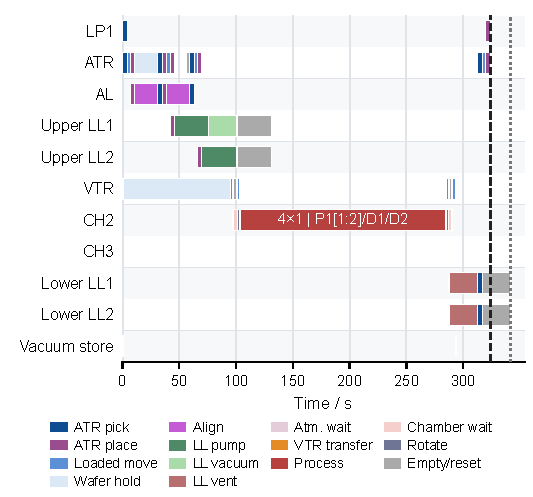
\includegraphics[width=\columnwidth]{Figure6}
\caption{Optimal product-completion schedule for two pure $4\times1$ products from the same LP. P1[1:2] denotes the two Pjob1 products; D1 and D2 are auxiliaries. Dashed and dotted lines mark product return at 324~s and the end of all occupancy at 342~s.}
\label{fig:small-optimal-gantt-cn}
\end{figure}


The two products form one PW pair and auxiliaries D1 and D2 form another, filling all four positions of CH2 for a 180~s exposure from 104 to 284~s. Products pass through ATR, AL, and the upper LL before VTR loads them. The auxiliary pair is loaded first, ensuring full occupancy when processing starts. After processing, products return through the lower LL to LP1, while auxiliaries return to vacuum storage at 294~s.

Both products return by 324~s, and lower-LL pressure reset continues until 342~s. The schedule shows auxiliary filling when fewer than four products are present and the complete supply and return routes, distinguishing product completion from equipment reset. The chamber executes one cycle and does not reach the cleaning threshold.

\subsubsection{A feasible two-chamber schedule for 16 products}
Figure~\ref{fig:current-defaults-gantt-cn} shows a feasible schedule for 16 pure $4\times1$ products. Each of the four LPs contains four products, all in Pjob1 and eligible for CH2 and CH3. Auxiliary inventory is eight and the cleaning threshold is three.


\begin{figure}[!htbp]
\centering
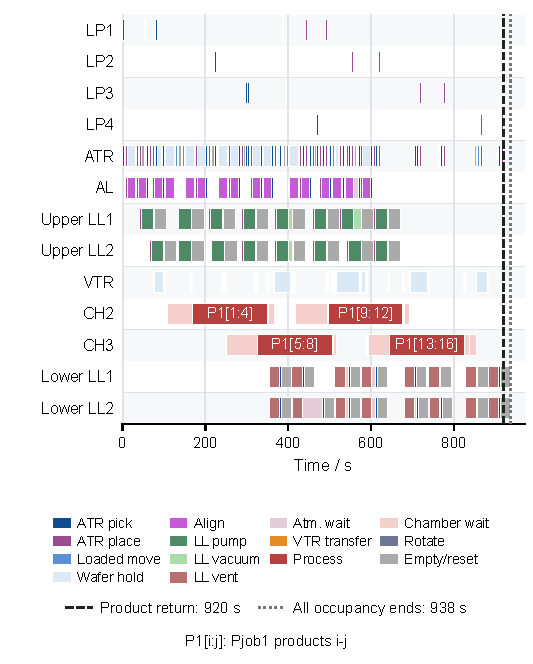
\includegraphics[width=\columnwidth]{Figure7}
\caption{Complete feasible resource schedule for 16 pure $4\times1$ products. LP1--LP4 each contain four Pjob1 products. Dashed and dotted lines mark product return at 920~s and the end of all occupancy at 938~s.}
\label{fig:current-defaults-gantt-cn}
\end{figure}


A preconstructed wafer-operation sequence is checked by substituting its pairs, chamber assignments, and event times into the complete model. The model contains 64 candidate PW pairs, 32 candidate cycles per chamber, 177905 variables, and 671864 constraints. All assignments satisfy chamber eligibility, finite capacities, nonprocessing residency limits, and nondecreasing release within each job. Independent event-time validation also passes.

Product completion is $C_{\max}=920$~s. Sixteen products form eight PW pairs and execute four full-occupancy cycles. CH2 processes Pjob1 products 1--4 at 170--350~s and 9--12 at 497--677~s. CH3 processes products 5--8 at 326--506~s and 13--16 at 645--825~s. Every product receives one 180~s exposure and returns to its original LP through the validated transport and LL sequence.

The 152 explicit events in Figure~\ref{fig:current-defaults-gantt-cn} cover LP pickups and returns, ATR, AL, upper and lower LLs, VTR, and both chambers. Chamber processing overlaps upstream and downstream transport; shared-robot and LL service orders constrain pair transitions. All products return by 920~s; lower-LL pressure reset ends at 938~s, 18~s later. Each chamber executes two cycles, below the cleaning threshold of three. Products fill every cycle, so no auxiliaries are borrowed. The schedule validates full occupancy and resource coordination across multiple products.

\FloatBarrier
\section{Conclusions}
This study addresses dual-source mixed-flow rotating-chamber CT scheduling, coordinating competition for shared resources among full occupancy, continuous processing, cleaning, and finite auxiliary-wafer circulation. Pjobs and source inventories encode products with common scheduling attributes, while two-wafer PW pairs link transport to chamber cycles. A common feasible region represents product pairing, chamber assignment, cleaning, auxiliary reuse, and resource orders. The two-stage MILP first minimizes completion of product returns to their original LPs, then preserves this upper bound and the principal discrete structure while improving waiting and production rhythm. This separates and coordinates batch completion efficiency and temporal quality.

RL-DMCT combines structured initialization with reinforcement-learning-based cut selection for time-limited solution of the model. SPBS exploits an existing schedule skeleton and progressively releases resource orders and other discrete decisions to improve the initial upper bound. Within HEM's hierarchical cut-selection framework, variable-role features and structural reranking jointly assess cut quality and structural complementarity, with beam search generating candidate sequences. Deterministic decoding recovers physical wafer identities and handling operations, followed by complete-model checks and independent event-time validation. The resulting procedure connects job encoding, joint optimization, and wafer-level schedule output.

The four experimental questions yield the following conclusions:
\begin{enumerate}[label=(\arabic*),leftmargin=*,itemsep=3pt,topsep=3pt]
\item Existing schedule structure improves time-limited feasible upper bounds. With common starts and a 300~s budget, fixed-structure optimization gives lower mean feasible bounds than direct joint search in all four mixed instances. Releasing discrete decisions yields further improvement in a small mixed instance. Existing structure therefore provides an effective starting point, while the benefit of broader search depends on the instance and budget allocation.
\item Product-completion optimization and timing refinement are complementary. All 30 paired stage comparisons reduce total waiting while preserving product completion. Rhythm-weight comparisons show that cycle regularity and waiting do not necessarily improve together; stage-two weights control their tradeoff.
\item Continuous-processing completion is constrained by finite auxiliary circulation. In single-product comparisons with equal total exposure time, increasing auxiliary inventory reduces the optimal $2\times2$ completion while leaving $4\times1$ unchanged. Auxiliary loan--return and cleaning schedules further validate the treatment of auxiliaries as reusable shared resources jointly scheduled with production chains, connecting full occupancy, continuous processing, and cleaning.
\item Initialization and learned cut selection make different contributions. Structured initialization is the main source of completion-time improvement in the two base mixed instances, with a consistent direction across three training seeds. With shared initial solutions, the complete cut-selection combination improves on HEM+SPBS and three component variants. Its gains depend on input structure, separation settings, and budget allocation.
\end{enumerate}
Model checks and event replay validate an optimal two-product schedule completing at 324~s and a feasible 16-product schedule completing at 920~s, translating model decisions into concrete transport, processing, and return sequences.

Future work will further improve time-limited solution quality under the coupled constraints of full occupancy, continuous processing, and finite auxiliary reuse. Product-completion bottlenecks will guide the choice of decisions to adjust. Structural agreement and disagreement among high-quality schedules will be used to select joint adjustment neighborhoods, with MILP repair and quality-guided search improving feasible upper bounds.

\section*{CRediT authorship contribution statement}
\textbf{Lincong Wei:} Conceptualization, Methodology, Software, Validation, Formal analysis, Investigation, Data curation, Visualization, Writing -- original draft, Writing -- review \& editing.
\textbf{Lizhen Shao:} Conceptualization, Methodology, Formal analysis, Writing -- review \& editing, Project administration.
\textbf{Wei Wang:} Formal analysis, Investigation, Writing -- review \& editing, Supervision. All authors reviewed and approved the final manuscript.

\section*{Funding}
This research did not receive any specific grant from funding agencies in the public, commercial, or not-for-profit sectors.

\section*{Declaration of competing interest}
The authors declare that they have no known competing financial interests or personal relationships that could have appeared to influence the work reported in this paper.

\section*{Data availability}
The data, mathematical instances, trained models, and software implementation supporting this study are available from the corresponding author upon reasonable request.

\section*{Declaration of generative AI and AI-assisted technologies in the manuscript preparation process}
During the preparation of this work, the authors used OpenAI ChatGPT and Codex to assist with language editing, Chinese--English translation, LaTeX consistency checks, and experimental visualization. After using these tools, the authors reviewed and edited the content as needed and take full responsibility for the content of the publication.

\footnotesize
\setlength{\bibsep}{0pt}
\begin{thebibliography}{32}
% JMS: Elsevier NLM/Vancouver, first-citation order. Generated by tools/format_jms_references.py.
\interlinepenalty=10000

\bibitem{appliedprecisioncvd}
Applied Materials. Producer XP Precision CVD.
n.d.
\url{https://www.appliedmaterials.com/us/en/product-library/producer-xp-precision-cvd.html} (accessed September 7, 2026).

\bibitem{gu2024applied}
Gu L, Wu N, Qiao Y, Zhang S, Li T. Scheduling cluster tools with multi-space process modules and a multi-finger-arm robot in wafer fabrication subject to wafer residency time constraints.
Appl Sci 2024;14:9490.
\url{https://doi.org/10.3390/app14209490}.

\bibitem{gu2024multifinger}
Gu L, Wu N, Qiao Y, Zhang S. Scheduling of {Multi-finger-robotic Cluster Tools} with {Multi-space Process Modules}.
In: 2024 International Conference on Networking, Sensing and Control ({ICNSC}). IEEE; 2024.
\url{https://doi.org/10.1109/ICNSC62968.2024.10760109}.

\bibitem{pan2018survey}
Pan CR, Zhou MC, Qiao Y, Wu NQ. Scheduling cluster tools in semiconductor manufacturing: Recent advances and challenges.
IEEE Trans Autom Sci Eng 2018;15:586--601.
\url{https://doi.org/10.1109/TASE.2016.2642997}.

\balance
\bibitem{perkinson1994throughput}
Perkinson TL, McLarty PK, Gyurcsik RS, Cavin RK. Single-wafer cluster tool performance: An analysis of throughput.
IEEE Trans Semicond Manuf 1994;7:369--73.
\url{https://doi.org/10.1109/66.311340}.

\bibitem{rostami2002optimal}
Rostami S, Hamidzadeh B. Optimal scheduling techniques for cluster tools with process-module and transport-module residency constraints.
IEEE Trans Semicond Manuf 2002;15:341--9.
\url{https://doi.org/10.1109/TSM.2002.801379}.

\bibitem{wu2010closedform}
Wu NQ, Zhou MC. A closed-form solution for schedulability and optimal scheduling of dual-arm cluster tools with wafer residency time constraint based on steady schedule analysis.
IEEE Trans Autom Sci Eng 2010;7:303--15.
\url{https://doi.org/10.1109/TASE.2008.2008633}.

\bibitem{qiao2012sojourn}
Qiao Y, Wu NQ, Zhou MC. Petri net modeling and wafer sojourn time analysis of single-arm cluster tools with residency time constraints and activity time variation.
IEEE Trans Semicond Manuf 2012;25:432--46.
\url{https://doi.org/10.1109/TSM.2012.2199338}.

\bibitem{qiao2014revisiting}
Qiao Y, Wu N, Zhou MC. Scheduling of dual-arm cluster tools with wafer revisiting and residency time constraints.
IEEE Trans Ind Inform 2014;10:286--300.
\url{https://doi.org/10.1109/TII.2013.2272702}.

\bibitem{wang2020multiple}
Wang J, Hu H, Pan C, Zhou Y, Li L. Scheduling dual-arm cluster tools with multiple wafer types and residency time constraints.
IEEE/CAA J Autom Sin 2020;7:776--89.
\url{https://doi.org/10.1109/JAS.2020.1003150}.

\bibitem{wang2025virtualcell}
Wang J, Liu C, Zhou MC, Abusorrah A. Virtual cell-based scheduling approach to single-robotic-arm cluster tools subject to wafer residency time constraints.
IEEE Trans Autom Sci Eng 2025;22:240--51.
\url{https://doi.org/10.1109/TASE.2024.3349380}.

\bibitem{yang2025miptwowafers}
Yang F, Li C, Zhen L, Zhang C, Wu N. Scheduling residency time-constrained single-armed cluster tools with two-wafer types via mixed integer programming model.
Expert Syst Appl 2025;288:128209.
\url{https://doi.org/10.1016/j.eswa.2025.128209}.

\bibitem{kim2013cleaning}
Kim H, Kim HJ, Lee JH, Lee TE. Scheduling dual-armed cluster tools with cleaning processes.
Int J Prod Res 2013;51:3671--87.
\url{https://doi.org/10.1080/00207543.2012.758392}.

\bibitem{yu2020delay}
Yu TS, Lee TE. Wafer delay analysis and control of dual-armed cluster tools with chamber cleaning operations.
Int J Prod Res 2020;58:434--47.
\url{https://doi.org/10.1080/00207543.2019.1593547}.

\bibitem{qiao2022binary}
Qiao Y, Lu Y, Li J, Zhang S, Wu N, Liu B. An efficient binary integer programming model for residency time-constrained cluster tools with chamber cleaning requirements.
IEEE Trans Autom Sci Eng 2022;19:1757--71.
\url{https://doi.org/10.1109/TASE.2021.3122576}.

\bibitem{li2022conditioncleaning}
Li C, Yang F, Zhen L. Efficient scheduling approaches to time-constrained single-armed cluster tools with condition-based chamber cleaning operations.
Int J Prod Res 2022;60:3555--68.
\url{https://doi.org/10.1080/00207543.2021.1926568}.

\bibitem{zhu2025failuredeadlock}
Zhu Q, Yuan J, Wang G, Hou Y. Scheduling a single-arm two-cluster tool with a process module failure subject to wafer residency time constraints.
IEEE Trans Autom Sci Eng 2025;22:667--79.
\url{https://doi.org/10.1109/TASE.2023.3275703}.

\bibitem{kim2025noncyclicdeadlock}
Kim D, Kim HJ. Noncyclic scheduling of cluster tools using deep reinforcement learning.
IEEE Trans Autom Sci Eng 2025;22:24009--23.
\url{https://doi.org/10.1109/TASE.2025.3632534}.

\bibitem{lee2018waiting}
Lee JH, Zhao C, Li J, Papadopoulos CT. Analysis, design, and control of {Bernoulli} production lines with waiting time constraints.
J Manuf Syst 2018;46:208--20.
\url{https://doi.org/10.1016/j.jmsy.2018.01.001}.

\bibitem{weng2022jit}
Weng W, Chen J, Zheng M, Fujimura S. Realtime scheduling heuristics for just-in-time production in large-scale flexible job shops.
J Manuf Syst 2022;63:64--77.
\url{https://doi.org/10.1016/j.jmsy.2022.01.006}.

\bibitem{sun2024manufacturing}
Sun L, Lyu P, Zhang X, Wu J, Wang Q, Ervin J, et~al. Machine learning technologies for semiconductor manufacturing.
In: 2024 Conference of Science and Technology for Integrated Circuits (CSTIC). IEEE; 2024, p. 1--7.
\url{https://doi.org/10.1109/CSTIC61820.2024.10532076}.

\bibitem{chen2020anomaly}
Chen CY, Chang SC, Liao DY. Equipment anomaly detection for semiconductor manufacturing by exploiting unsupervised learning from sensory data.
Sensors 2020;20:5650.
\url{https://doi.org/10.3390/s20195650}.

\bibitem{biebl2020maintenance}
Biebl F, Glawar R, Jalali A, Ansari F, Haslhofer B, de~Boer P, et~al. A conceptual model to enable prescriptive maintenance for etching equipment in semiconductor manufacturing.
Procedia CIRP 2020;88:64--9.
\url{https://doi.org/10.1016/j.procir.2020.05.012}.

\bibitem{rahmani2014robust}
Rahmani D, Heydari M. Robust and stable flow shop scheduling with unexpected arrivals of new jobs and uncertain processing times.
J Manuf Syst 2014;33:84--92.
\url{https://doi.org/10.1016/j.jmsy.2013.03.004}.

\bibitem{kim2025adaptivecluster}
Kim HJ, Lee JH. Scheduling cluster tools for concurrent processing: Deep reinforcement learning with adaptive search.
IEEE Trans Autom Sci Eng 2025;22:3783--96.
\url{https://doi.org/10.1109/TASE.2024.3399818}.

\bibitem{tang2020cut}
Tang Y, Agrawal S, Faenza Y. Reinforcement learning for integer programming: Learning to cut.
In: Proceedings of the 37th International Conference on Machine Learning. PMLR; 2020, p. 9367--76.
\url{https://proceedings.mlr.press/v119/tang20a.html}.

\bibitem{huang2022cutranking}
Huang Z, Wang K, Liu F, Zhen HL, Zhang W, Yuan M, et~al. Learning to select cuts for efficient mixed-integer programming.
Pattern Recognit 2022;123:108353.
\url{https://doi.org/10.1016/j.patcog.2021.108353}.

\bibitem{paulus2022looking}
Paulus MB, Zarpellon G, Krause A, Charlin L, Maddison C. Learning to cut by looking ahead: Cutting plane selection via imitation learning.
In: Proceedings of the 39th International Conference on Machine Learning. PMLR; 2022, p. 17584--600.
\url{https://proceedings.mlr.press/v162/paulus22a.html}.

\bibitem{wang2023hem}
Wang Z, Li X, Wang J, Kuang Y, Yuan M, Zeng J, et~al. Learning cut selection for mixed-integer linear programming via hierarchical sequence model.
In: Proceedings of the Eleventh International Conference on Learning Representations. 2023.
\url{https://openreview.net/forum?id=Zob4P9bRNcK}.

\bibitem{krause2014submodular}
Krause A, Golovin D. Submodular function maximization.
In: Tractability: Practical Approaches to Hard Problems. Cambridge University Press; 2014.
\url{https://las.inf.ethz.ch/bibtexbrowser.php?bib=laspub.bib\&key=krause14survey}.

\bibitem{achterberg2009scip}
Achterberg T. {SCIP}: Solving constraint integer programs.
Math Program Comput 2009;1:1--41.
\url{https://doi.org/10.1007/s12532-008-0001-1}.

\bibitem{bestuzheva2023scip}
Bestuzheva K, Besan{\c{c}}on M, Chen WK, Chmiela A, Donkiewicz T, van Doornmalen J, et~al. Enabling research through the {SCIP} optimization suite 8.0.
ACM Trans Math Softw 2023;49:22:1--22:21.
\url{https://doi.org/10.1145/3585516}.

\end{thebibliography}

\end{document}


